\documentclass[10pt,a4paper,french]{beamer}
\usepackage{cmap}
\usepackage[T1]{fontenc}
\usepackage[utf8]{inputenc}
\usepackage[french]{babel}
\usepackage{siunitx}
\usepackage{graphicx}
\usepackage{amsmath}
\usetheme{Darmstadt}
\setbeamertemplate{footline}[frame number]
\newcommand*\diff{\mathop{}\!\mathrm{d}}
\usepackage{xcolor,colortbl}
\usepackage{subfig}
\usepackage{tikz}
\usepackage{lmodern}
\usepackage{chemist}
\usepackage{etoolbox}
\usetikzlibrary{arrows,shapes,backgrounds}
\definecolor{Orange}{HTML}{FFDD00}
\definecolor{Orange2}{HTML}{FFC000}
\definecolor{Green}{HTML}{8FB73E}
\definecolor{Green2}{HTML}{4EA700}
\definecolor{Red}{HTML}{EF4123}
\definecolor{Red2}{HTML}{EF2300}
%\usefonttheme[onlylarge]{structuresmallcapsserif}
%\usefonttheme[onlysmall]{structurebold}
\usepackage{etoolbox}
\usepackage{pgfplots}
\pgfplotsset{compat=newest}
\usepgfplotslibrary{external,colormaps} 
\useinnertheme{circles}
\newenvironment<>{vert}[1]{%
	\setbeamercolor{block title}{fg=black,bg=Green2}%
	\setbeamercolor{block body}{fg=black, bg=Green}%
	\begin{block}#2{#1}}{\end{block}}
\newenvironment<>{rouge}[1]{%
	\setbeamercolor{block title}{fg=black,bg=Red2}%
	\setbeamercolor{block body}{fg=black, bg=Red}%
	\begin{block}#2{#1}}{\end{block}}

\addtobeamertemplate{proof begin}{%
	\setbeamercolor{block title}{fg=black,bg=red!50!white}
	\setbeamercolor{block body}{fg=red, bg=red!30!white}
}{}
\setbeamertemplate{navigation symbols}{}
\newcommand{\includetex}[1]
{%
	\tikzsetnextfilename{#1}%
	\input{#1.tex}%
}

\makeatletter
\setbeamertemplate{footline}
{
	\leavevmode%
	\hbox{%
		\begin{beamercolorbox}[wd=.333333\paperwidth,ht=2.25ex,dp=1ex,center]{author in head/foot}%
			\usebeamerfont{author in head/foot}\insertsection
		\end{beamercolorbox}%
		\begin{beamercolorbox}[wd=.333333\paperwidth,ht=2.25ex,dp=1ex,center]{title in head/foot}%
			\usebeamerfont{title in head/foot}\insertsubsection
		\end{beamercolorbox}%
		\begin{beamercolorbox}[wd=.333333\paperwidth,ht=2.25ex,dp=1ex,right]{date in head/foot}%
			\usebeamerfont{date in head/foot}\insertshortdate{}\hspace*{2em}
			\insertframenumber{} / \inserttotalframenumber\hspace*{2ex} 
	\end{beamercolorbox}}%
	\vskip0pt%
}
\makeatother

\DeclareSIUnit{\bits}{bits}
\DeclareSIUnit{\hit}{Hits}
\DeclareSIUnit{\hitt}{Hit}
\DeclareSIUnit{\strip}{Strip}
\usepackage{appendixnumberbeamer}
% Add total frame count to slides, optional. From Stefan,
% http://www.latex-community.org/forum/viewtopic.php?f=4&t=2173
\expandafter\def\expandafter\insertshorttitle\expandafter{%
	\insertshorttitle\hfill\insertframenumber\,/\,\inserttotalframenumber}

\mode<presentation>
\title{Caractérisation de détecteurs à plaques résistives de verres de basse résistivité en vue de la mise à niveau de CMS} 
\author{Lagarde François}
\date{20 Octobre 2017}
\institute{Institut de Physique Nucléaire de Lyon}

% logo of my university
\titlegraphic{%
	
\includegraphics[width=2.5cm]{logo}\hspace*{4.75cm}~%
	
\includegraphics[width=2cm]{logo2}
}

\begin{document}
	\tikzstyle{every picture}+=[remember picture]
	\tikzstyle{na} = [baseline=-.5ex]
	%titre
	\begin{frame}
		\titlepage
	\end{frame}
	%sommaire
	\begin{frame}
		\frametitle{Sommaire}
		\tableofcontents[hideallsubsections]
	\end{frame}

	\section{Contexte}
	\subsection{Les particules élémentaires, le Modèle Standard}
	\begin{frame}
	\begin{columns}
		\column{.6\textwidth}
		\begin{center}
		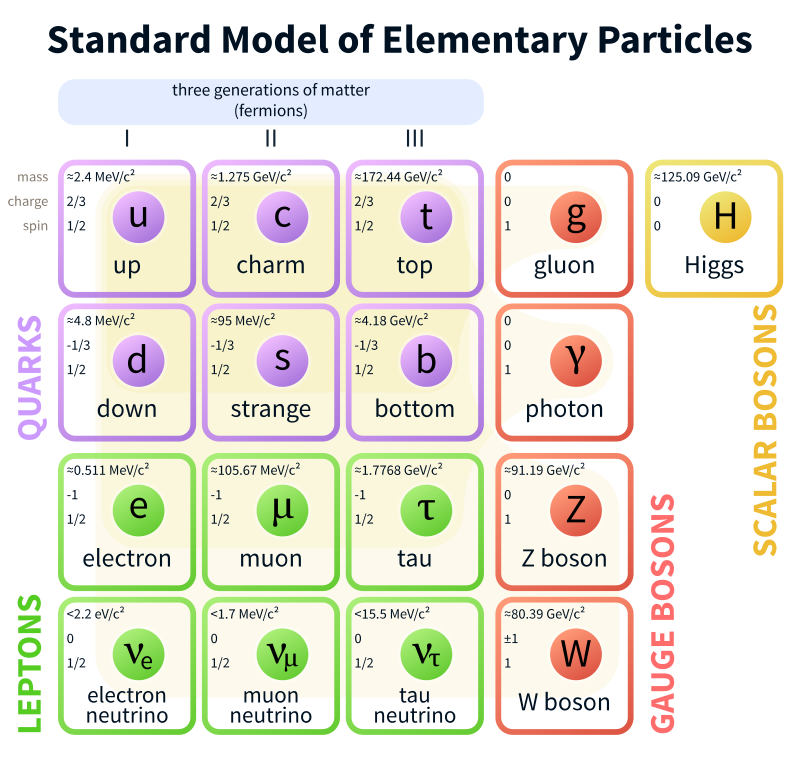
\includegraphics[height=0.6\textheight]{bestiaire.png}
		\end{center}
		\column{.45\textwidth}
		\begin{block}{\centering Fermions (Spin demi-entier)}
			\setlength\abovedisplayskip{0pt}
			\begin{itemize}
				\item 6 quarks (anti-quarks)
				\item 6 leptons (anti-leptons)
			\end{itemize}
		\end{block}
		\begin{block}{\centering Bosons (Spin entier)}
			\setlength\abovedisplayskip{0pt}
			%\hspace*{.1\linewidth}\begin{minipage}{.8\linewidth}
			%\begin{block}{Médiateurs des interactions}
				\begin{itemize}
					\item 8 gluons (force forte)
					\item $\gamma$ (électromagnétisme)
					\item $Z^{0}$ $W^{\pm}$ (force électrofaible)
				%\end{itemize}
			%\end{block}
			%\end{minipage}
			%\begin{itemize}
				\item Boson de Higgs
			\end{itemize}
		\end{block}
	\end{columns}
	\begin{block}{\centering Lagrangien du Modèle Standard}
		\begin{equation}
		\only<1>{\mathcal{L_{MS}}=\textcolor{red}{\mathcal{L}_{\mathrm{Yang-Mills}}}+\mathcal{L}_{\mathrm{Dirac}}+\mathcal{L}_{\mathrm{Higgs}}+\mathcal{L}_{\mathrm{Yukawa}}}
		\only<2>{\mathcal{L_{MS}}=\mathcal{L}_{\mathrm{Yang-Mills}}+\textcolor{red}{\mathcal{L}_{\mathrm{Dirac}}}+\mathcal{L}_{\mathrm{Higgs}}+\mathcal{L}_{\mathrm{Yukawa}}}
		\only<3>{\mathcal{L_{MS}}=\mathcal{L}_{\mathrm{Yang-Mills}}+\mathcal{L}_{\mathrm{Dirac}}+\textcolor{red}{\mathcal{L}_{\mathrm{Higgs}}}+\mathcal{L}_{\mathrm{Yukawa}}}
		\only<4>{\mathcal{L_{MS}}=\mathcal{L}_{\mathrm{Yang-Mills}}+\mathcal{L}_{\mathrm{Dirac}}+\mathcal{L}_{\mathrm{Higgs}}+\textcolor{red}{\mathcal{L}_{\mathrm{Yukawa}}}}
		\end{equation}
		\begin{overlayarea}{0.99\textwidth}{1cm}
		\begin{itemize}
			{\only<1>{\color{red}\item $\mathcal{L}_{\mathrm{Yang-Mills}}$ Partie cinétique des champs de jauges.}}
			{\only<2>{\color{red}\item $\mathcal{L}_{\mathrm{Dirac}}$ Interactions entre fermions et bosons de jauges.}}
			{\only<3>{\color{red}\item $\mathcal{L}_{\mathrm{Higgs}}$ Donne la masse aux bosons $Z^{0}$,$W^{\pm}$.}}
			{\only<4>{\color{red}\item $\mathcal{L}_{\mathrm{Yukawa}}$ Interactions entre le boson de Higgs et les fermions.}}
		\end{itemize}
		\end{overlayarea}
	\end{block}
\end{frame}
	\subsection{Le complexe d'accélération du CERN}	
	\begin{frame}
	    	\begin{columns}
	    		\column{.5\textwidth}
	    		\begin{center}
	    		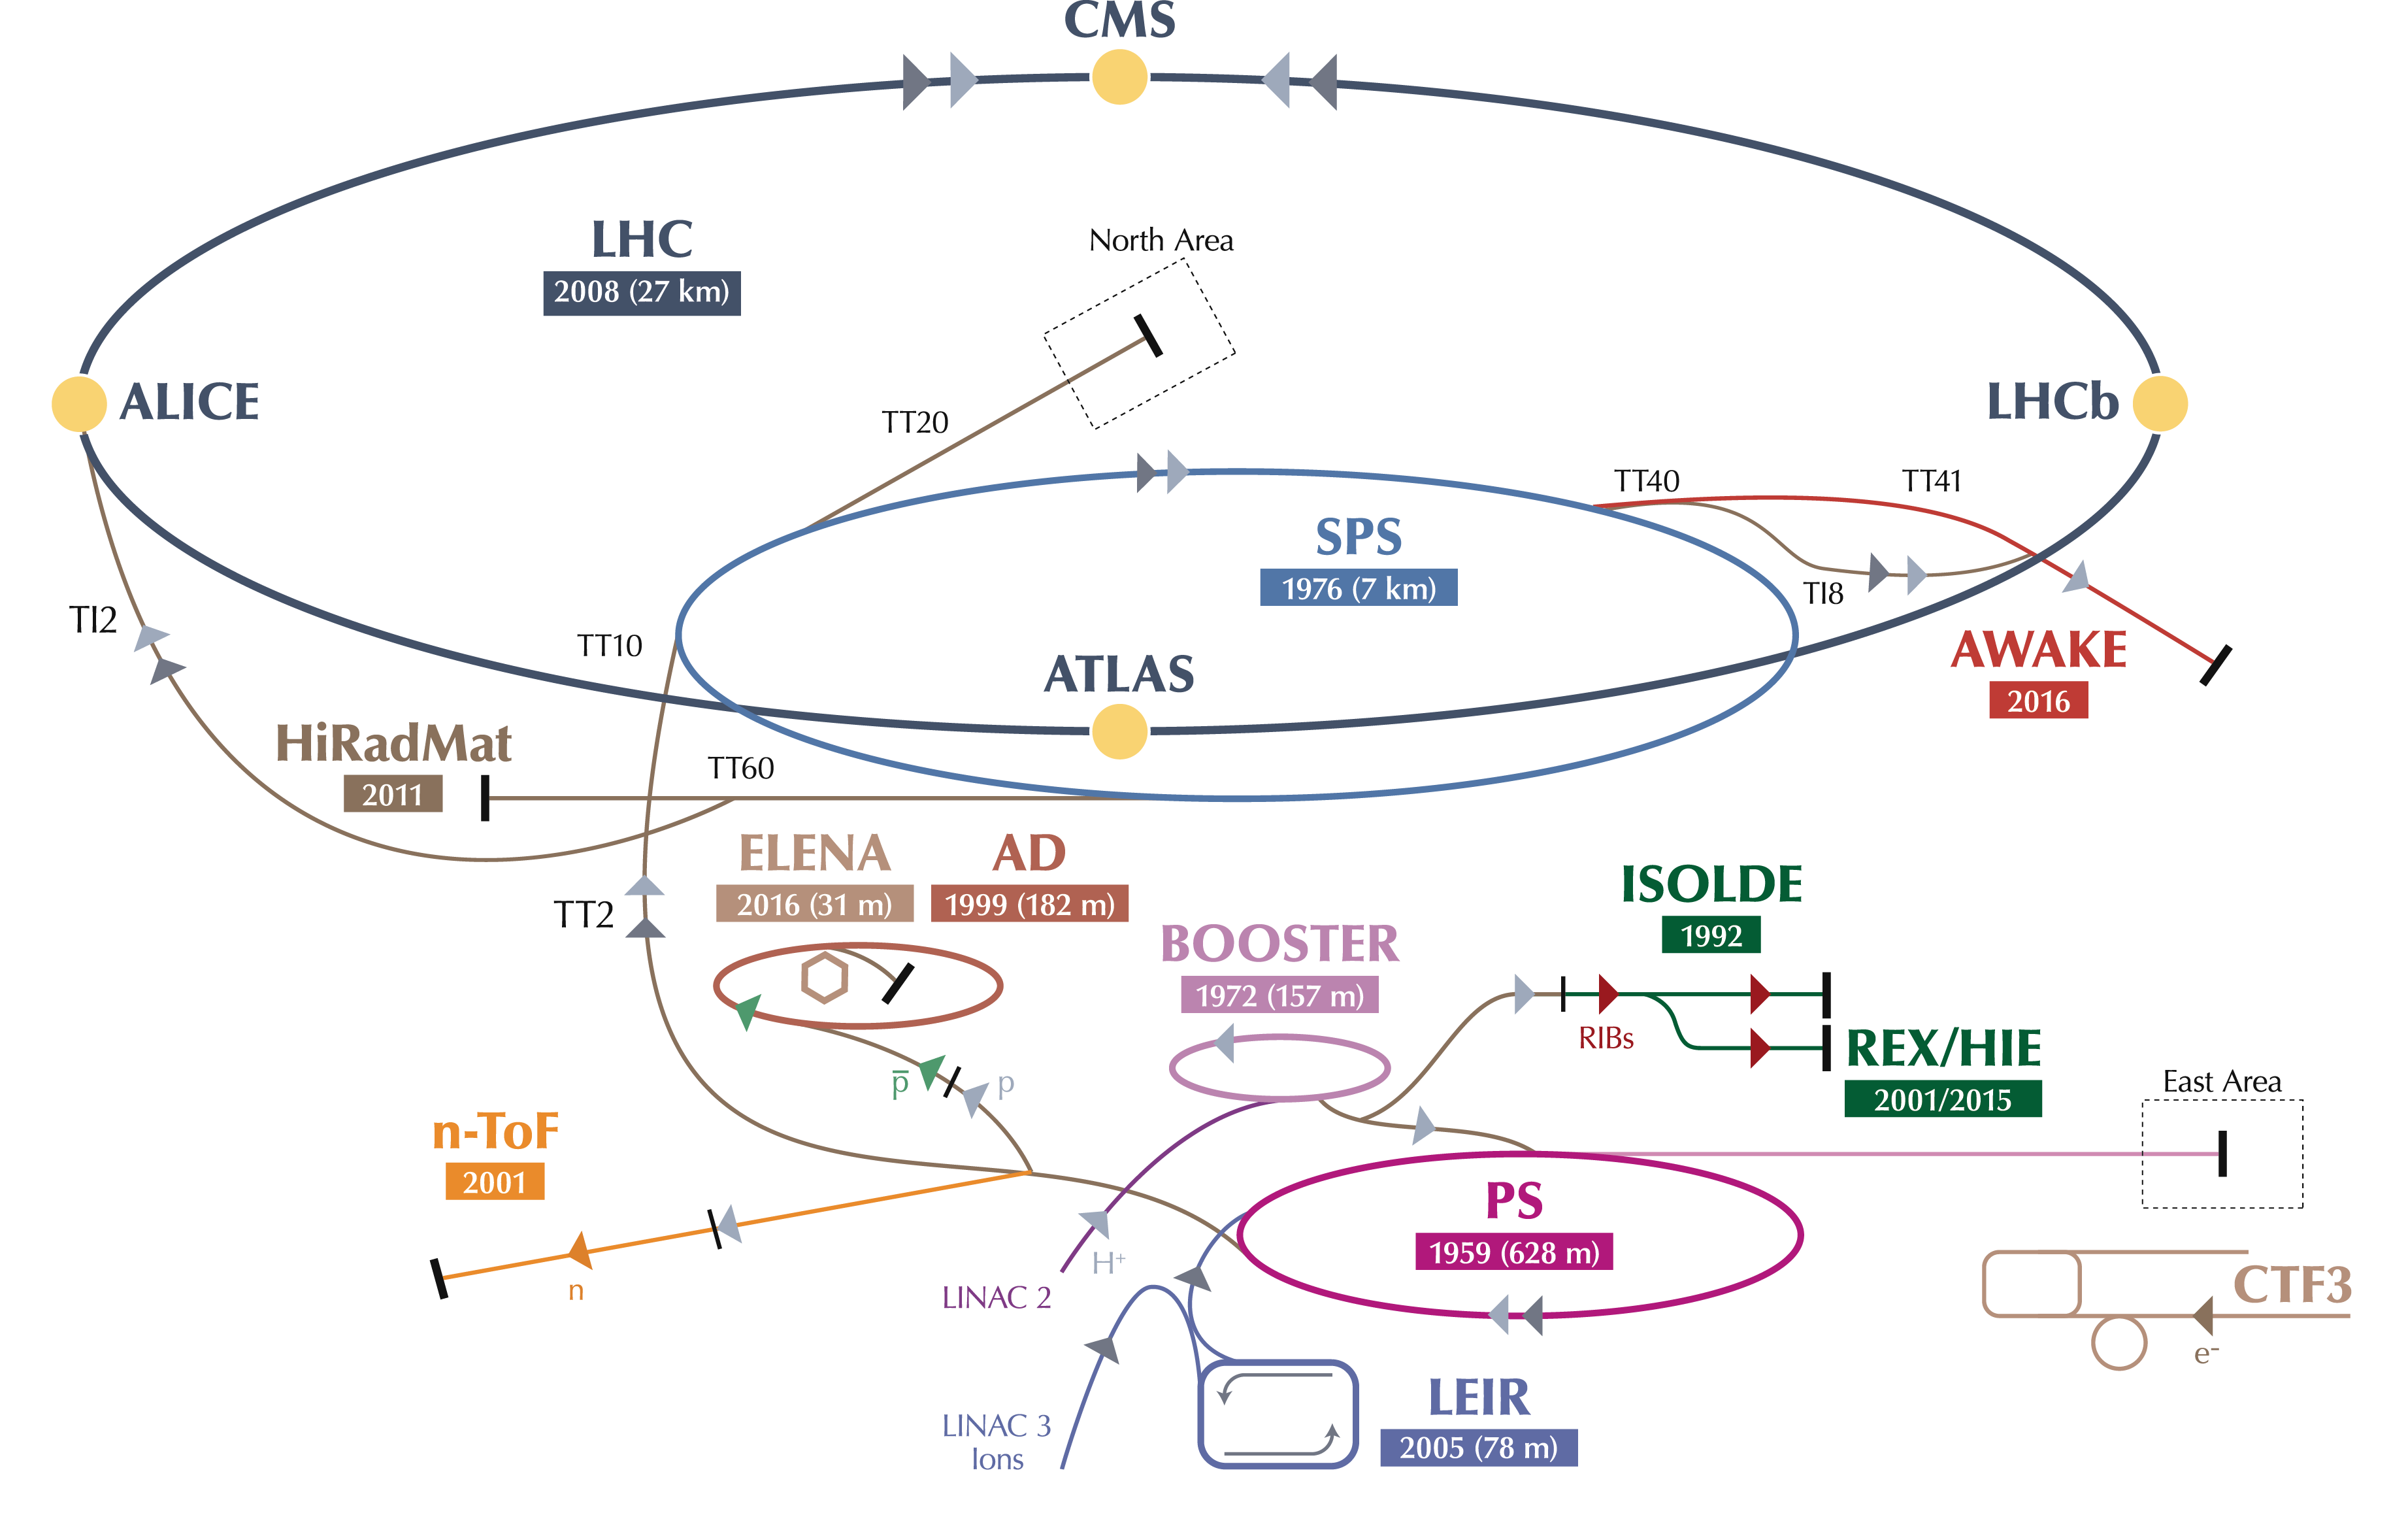
\includegraphics[width=1.1\textwidth]{complexe.png}
	    		\end{center}
	    		\column{.5\textwidth}
	    		\begin{block}{\centering Pour les collisions proton-proton}
	    			\begin{itemize}
	    				\item LINAC 2 ($\SI{50}{\mega\eV}$)
	    				\item BOOSTER ($\SI{1.4}{\giga\eV}$)
	    				\item Synchrotron à protons (PS) ($\SI{25}{\giga\eV}$)
	    				\item SuperSynchrotron à protons (SPS) ($\SI{450}{\giga\eV}$)
	    				\item Large Hadron Collider (LHC) ($\SI{7}{\tera\eV}$)
	    			\end{itemize}
	    		\end{block}
	    \end{columns}
	\end{frame}
	\subsection{Le LHC}
	\begin{frame}
	\begin{columns}
		\column{.5\textwidth}
		\begin{center}
		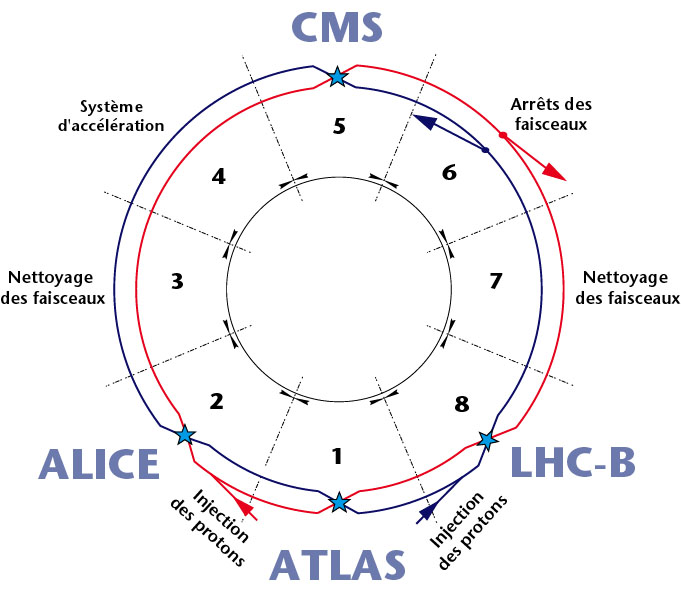
\includegraphics[width=0.99\textwidth]{lhc-schematic.jpg}
		\end{center}
		\column{.65\textwidth}
		\begin{block}{\centering Le LHC}
			\begin{itemize}
				\item Collisions p-p, ion-ion, ion-proton
				\item \SI{27}{\kilo\meter} de circonférence
				\item 1 collision toutes les \SI{25}{\nano\second}
				\item $\sqrt{s_{pp}}=\SI{14}{\tera\eV}$
				\item Luminosité instantanée $\sim\SI{e34}{\per\square\centi\meter\per\second}$
			\end{itemize}
		\end{block}
	\end{columns}
	\begin{block}{\centering Quatre expériences principales}
			\begin{figure}
			\subfloat[ALICE]{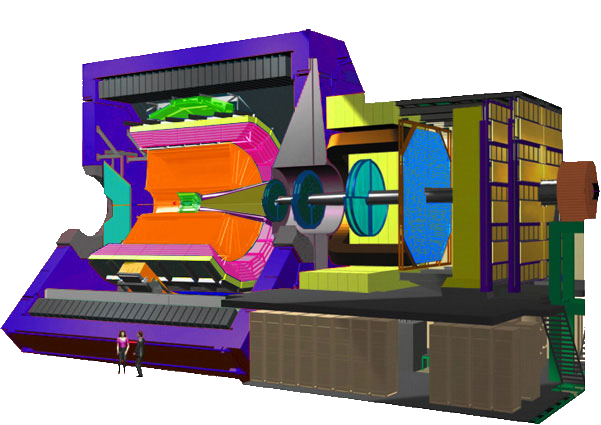
\includegraphics[width=.2\linewidth]{alice.png}}
			\hfill
			\subfloat[ATLAS]{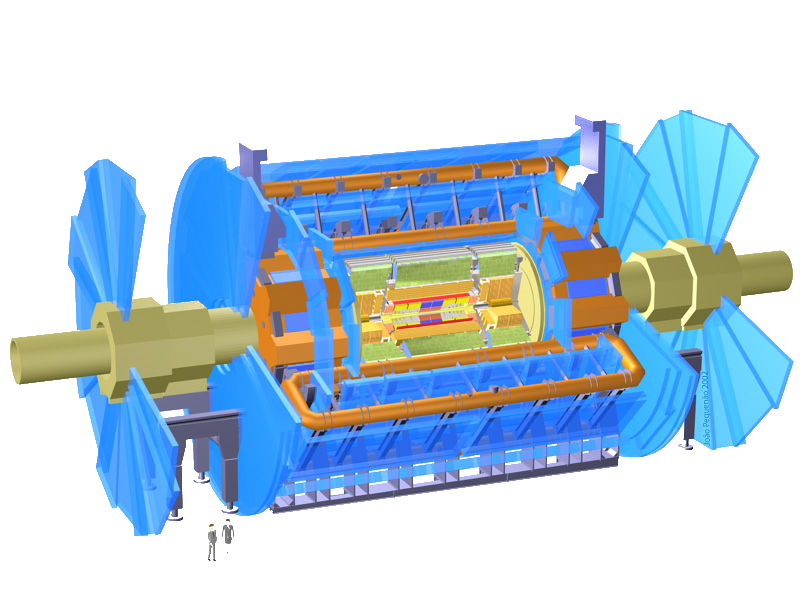
\includegraphics[width=.2\linewidth]{atlas.png}}
			\hfill
			\subfloat[LHC-b]{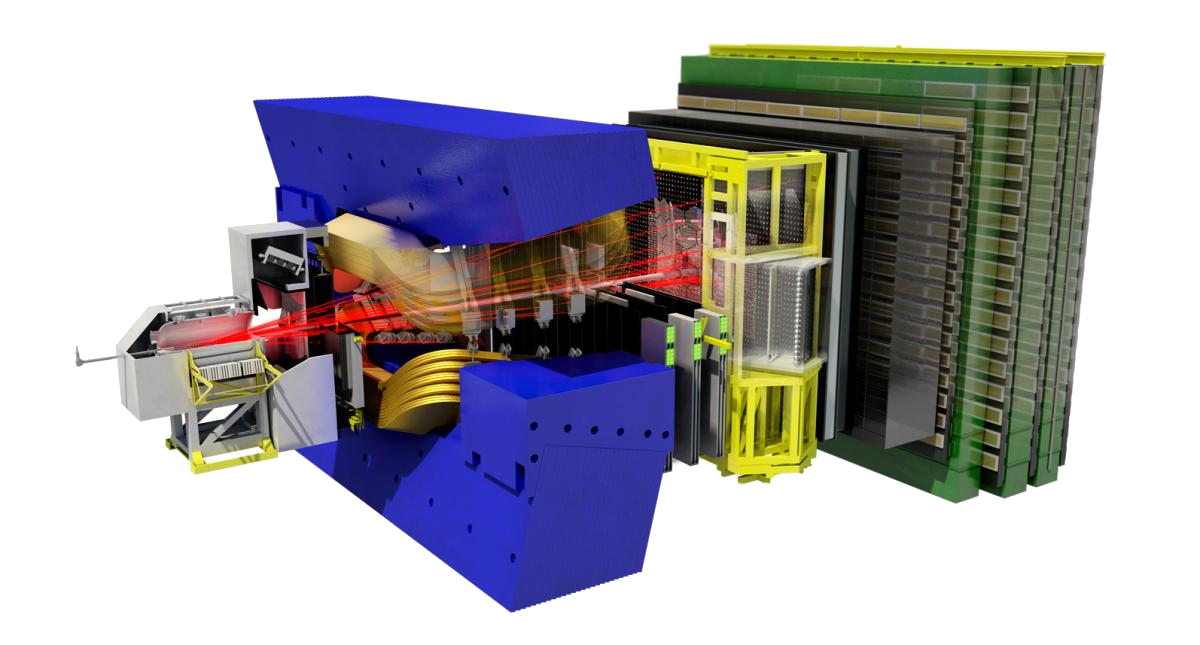
\includegraphics[width=.2\linewidth]{lhcb.png}}
			\hfill
			\subfloat[CMS]{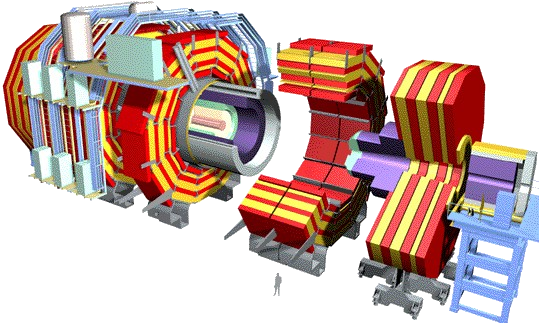
\includegraphics[width=.2\linewidth]{cms.png}}
		\end{figure}
	\end{block}
	\end{frame}
    \subsection{Le HL-LHC}
    \begin{frame}
    \begin{columns}
    	\column{.6\textwidth}
   	\begin{block}{\centering Le HL-LHC (2023-2035)}
   	Augmenter la luminosité $\mathcal{L}(t)$ ($\times$ \SIrange{5}{7}{}):
   	\begin{equation}
   	N_{event}=\int_{t=0}^{t=T} \mathcal{L}(t)\sigma \mathrm dt
   	\end{equation}
   	\begin{itemize}
   		\item $\sigma$ est la section efficace du processus
   		\item $T$ la durée de prise de données
   		\item $\mathcal{L}$ la luminosité instantanée délivrée par le LHC.
   	\end{itemize}
     	\end{block}
   \column{.5\textwidth}
   \begin{center}
   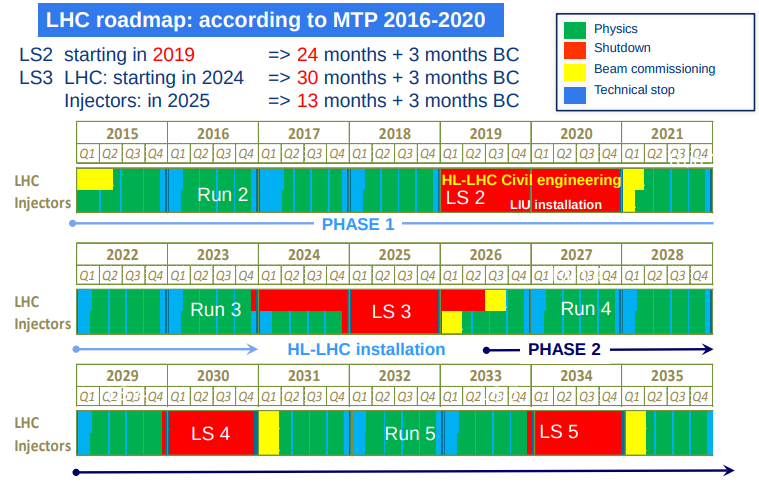
\includegraphics[width=1\textwidth]{roadmap.png}
   \end{center}
   	\end{columns}
   \visible<2>
  	{
  		\begin{block}{}
  		{\color{red}Augmentation de la luminosité $\Rightarrow$ Augmentation du \textit{pile-up} ($\sim$ 140-200) et du flux de particules dans les détecteurs $\Rightarrow$ Mise à niveau de CMS.}
  		\end{block}
  	}
	\end{frame}
	\subsection{Le Compact Muon Solenoid (CMS)}
	\begin{frame}
	\begin{block}{\centering Le Compact Muon Solenoid (CMS)}
		\only<1>{\begin{center}
		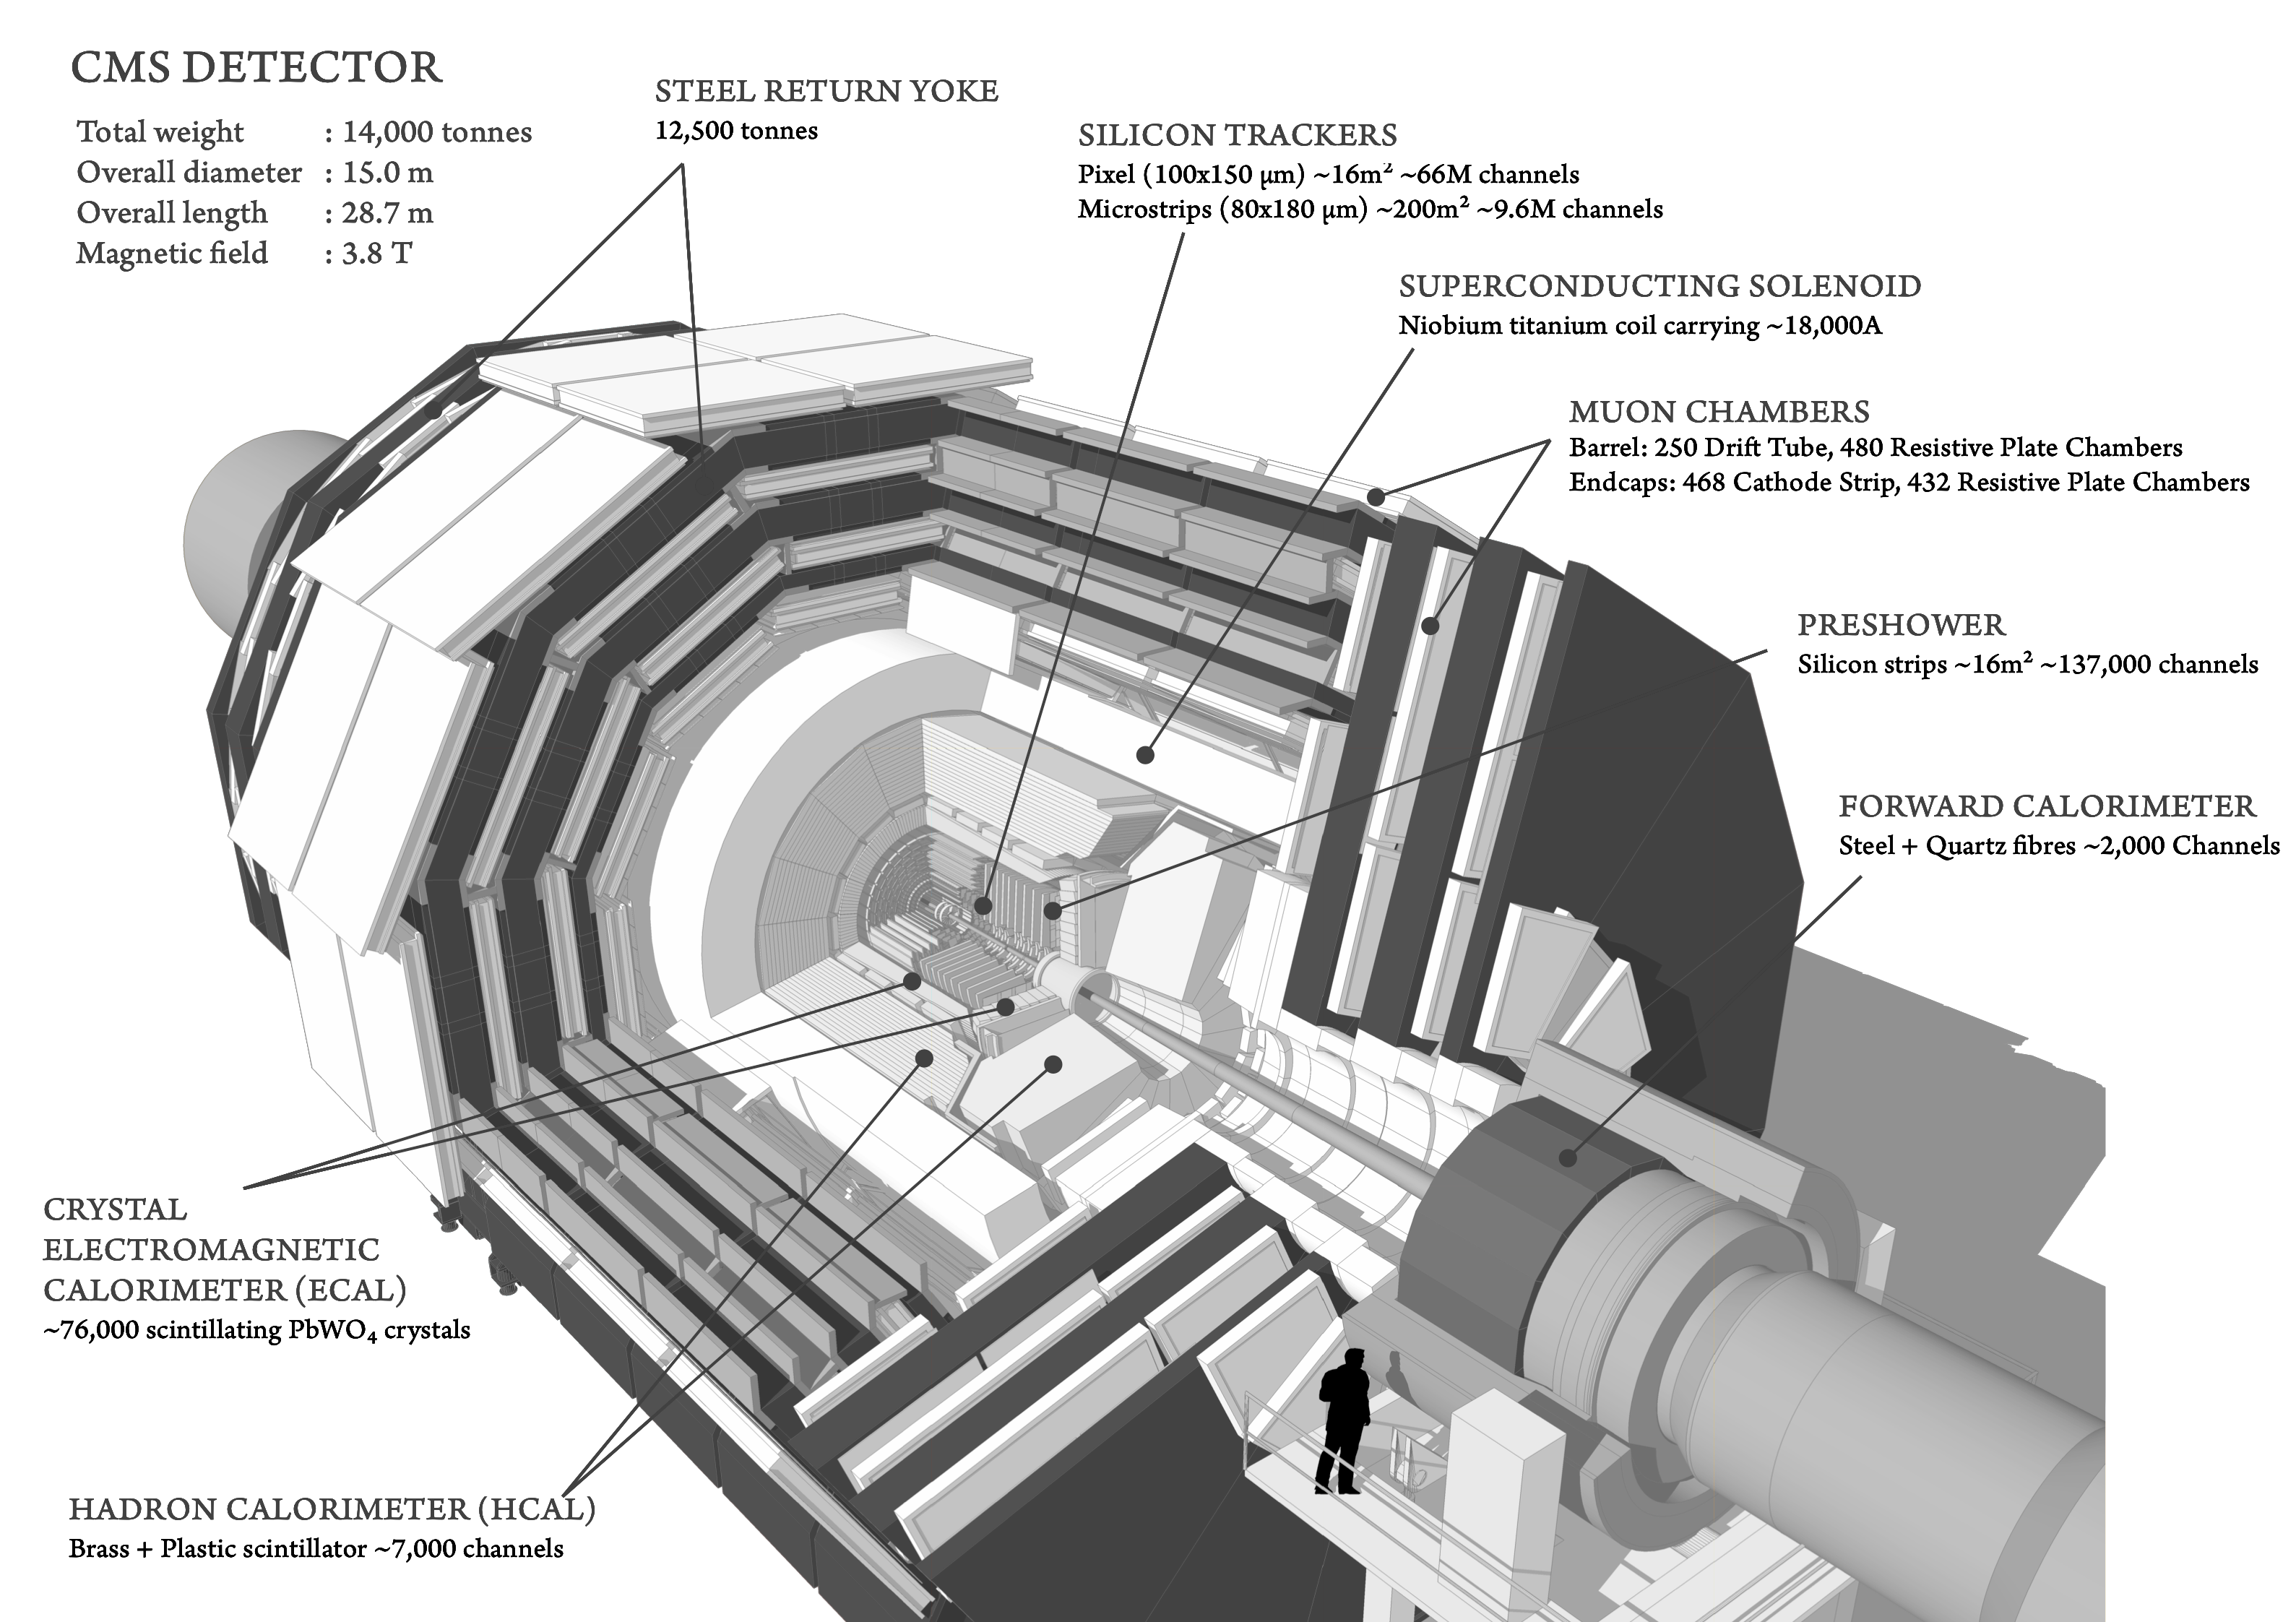
\includegraphics[width=0.95\textwidth]{cms_empty.png}
		\end{center}}
		\only<2>{\begin{center}
		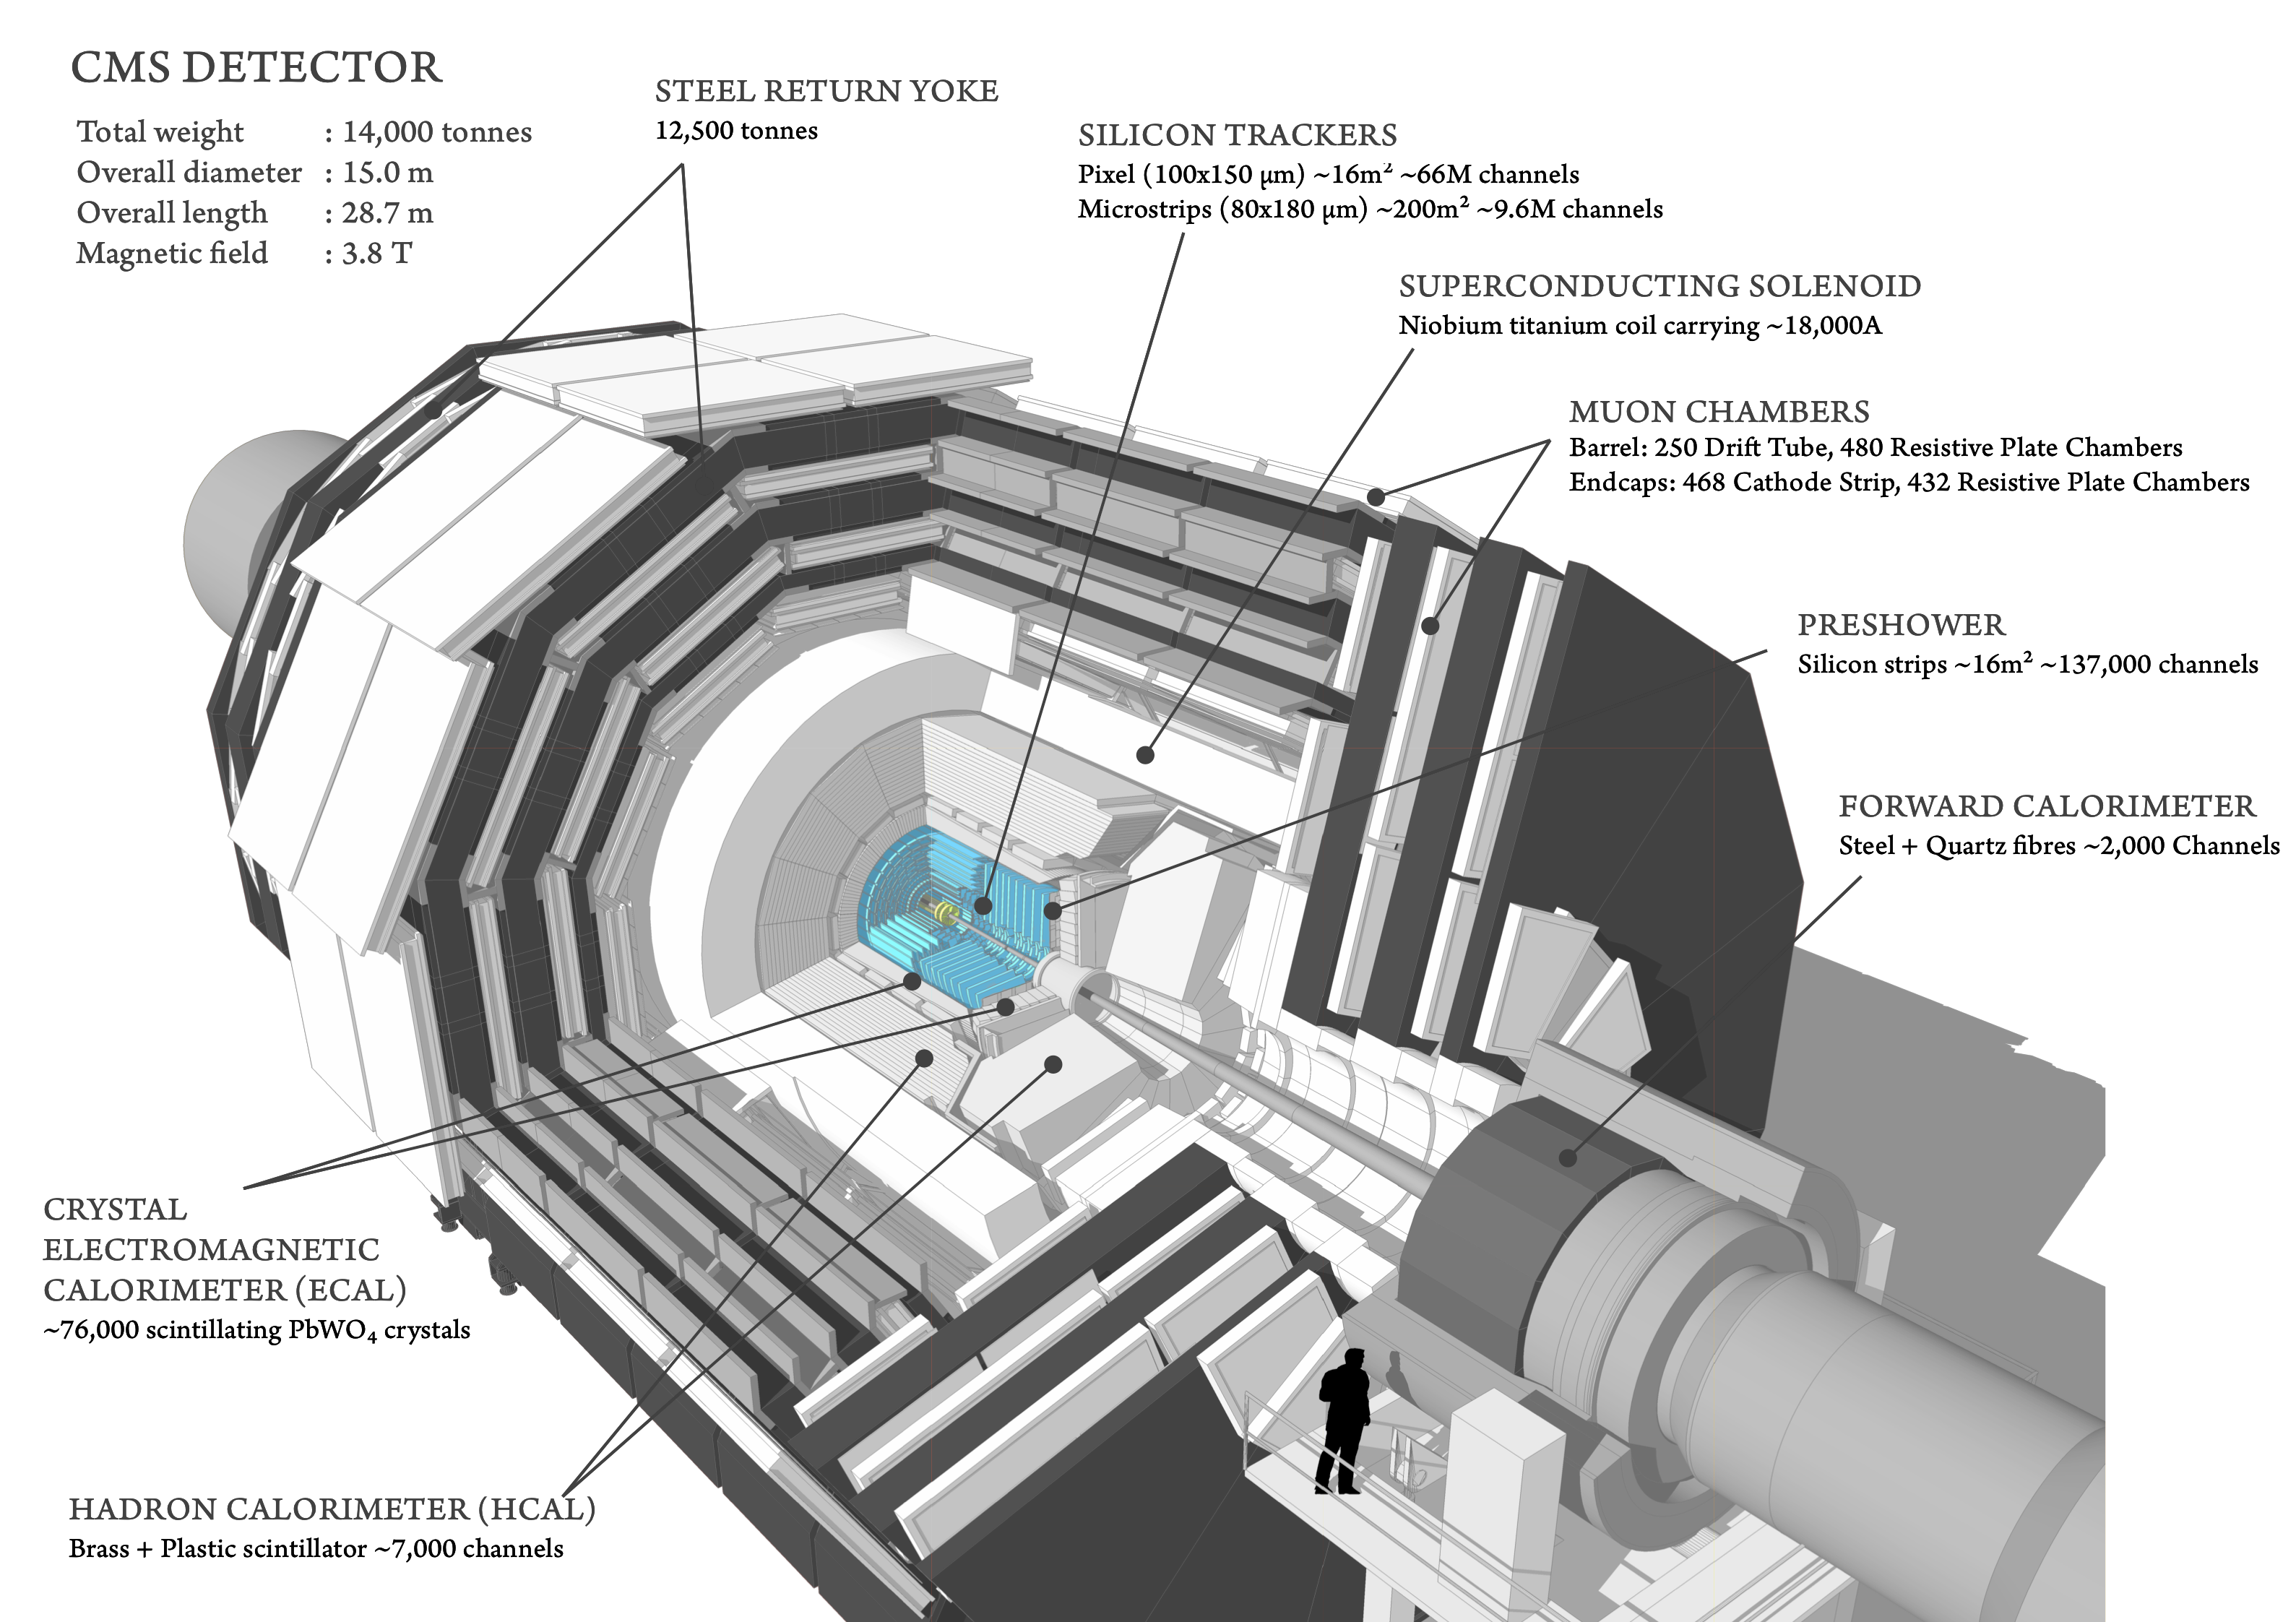
\includegraphics[width=0.95\textwidth]{cms_tracker.png}
	\end{center}}
		\only<3>{\begin{center}
		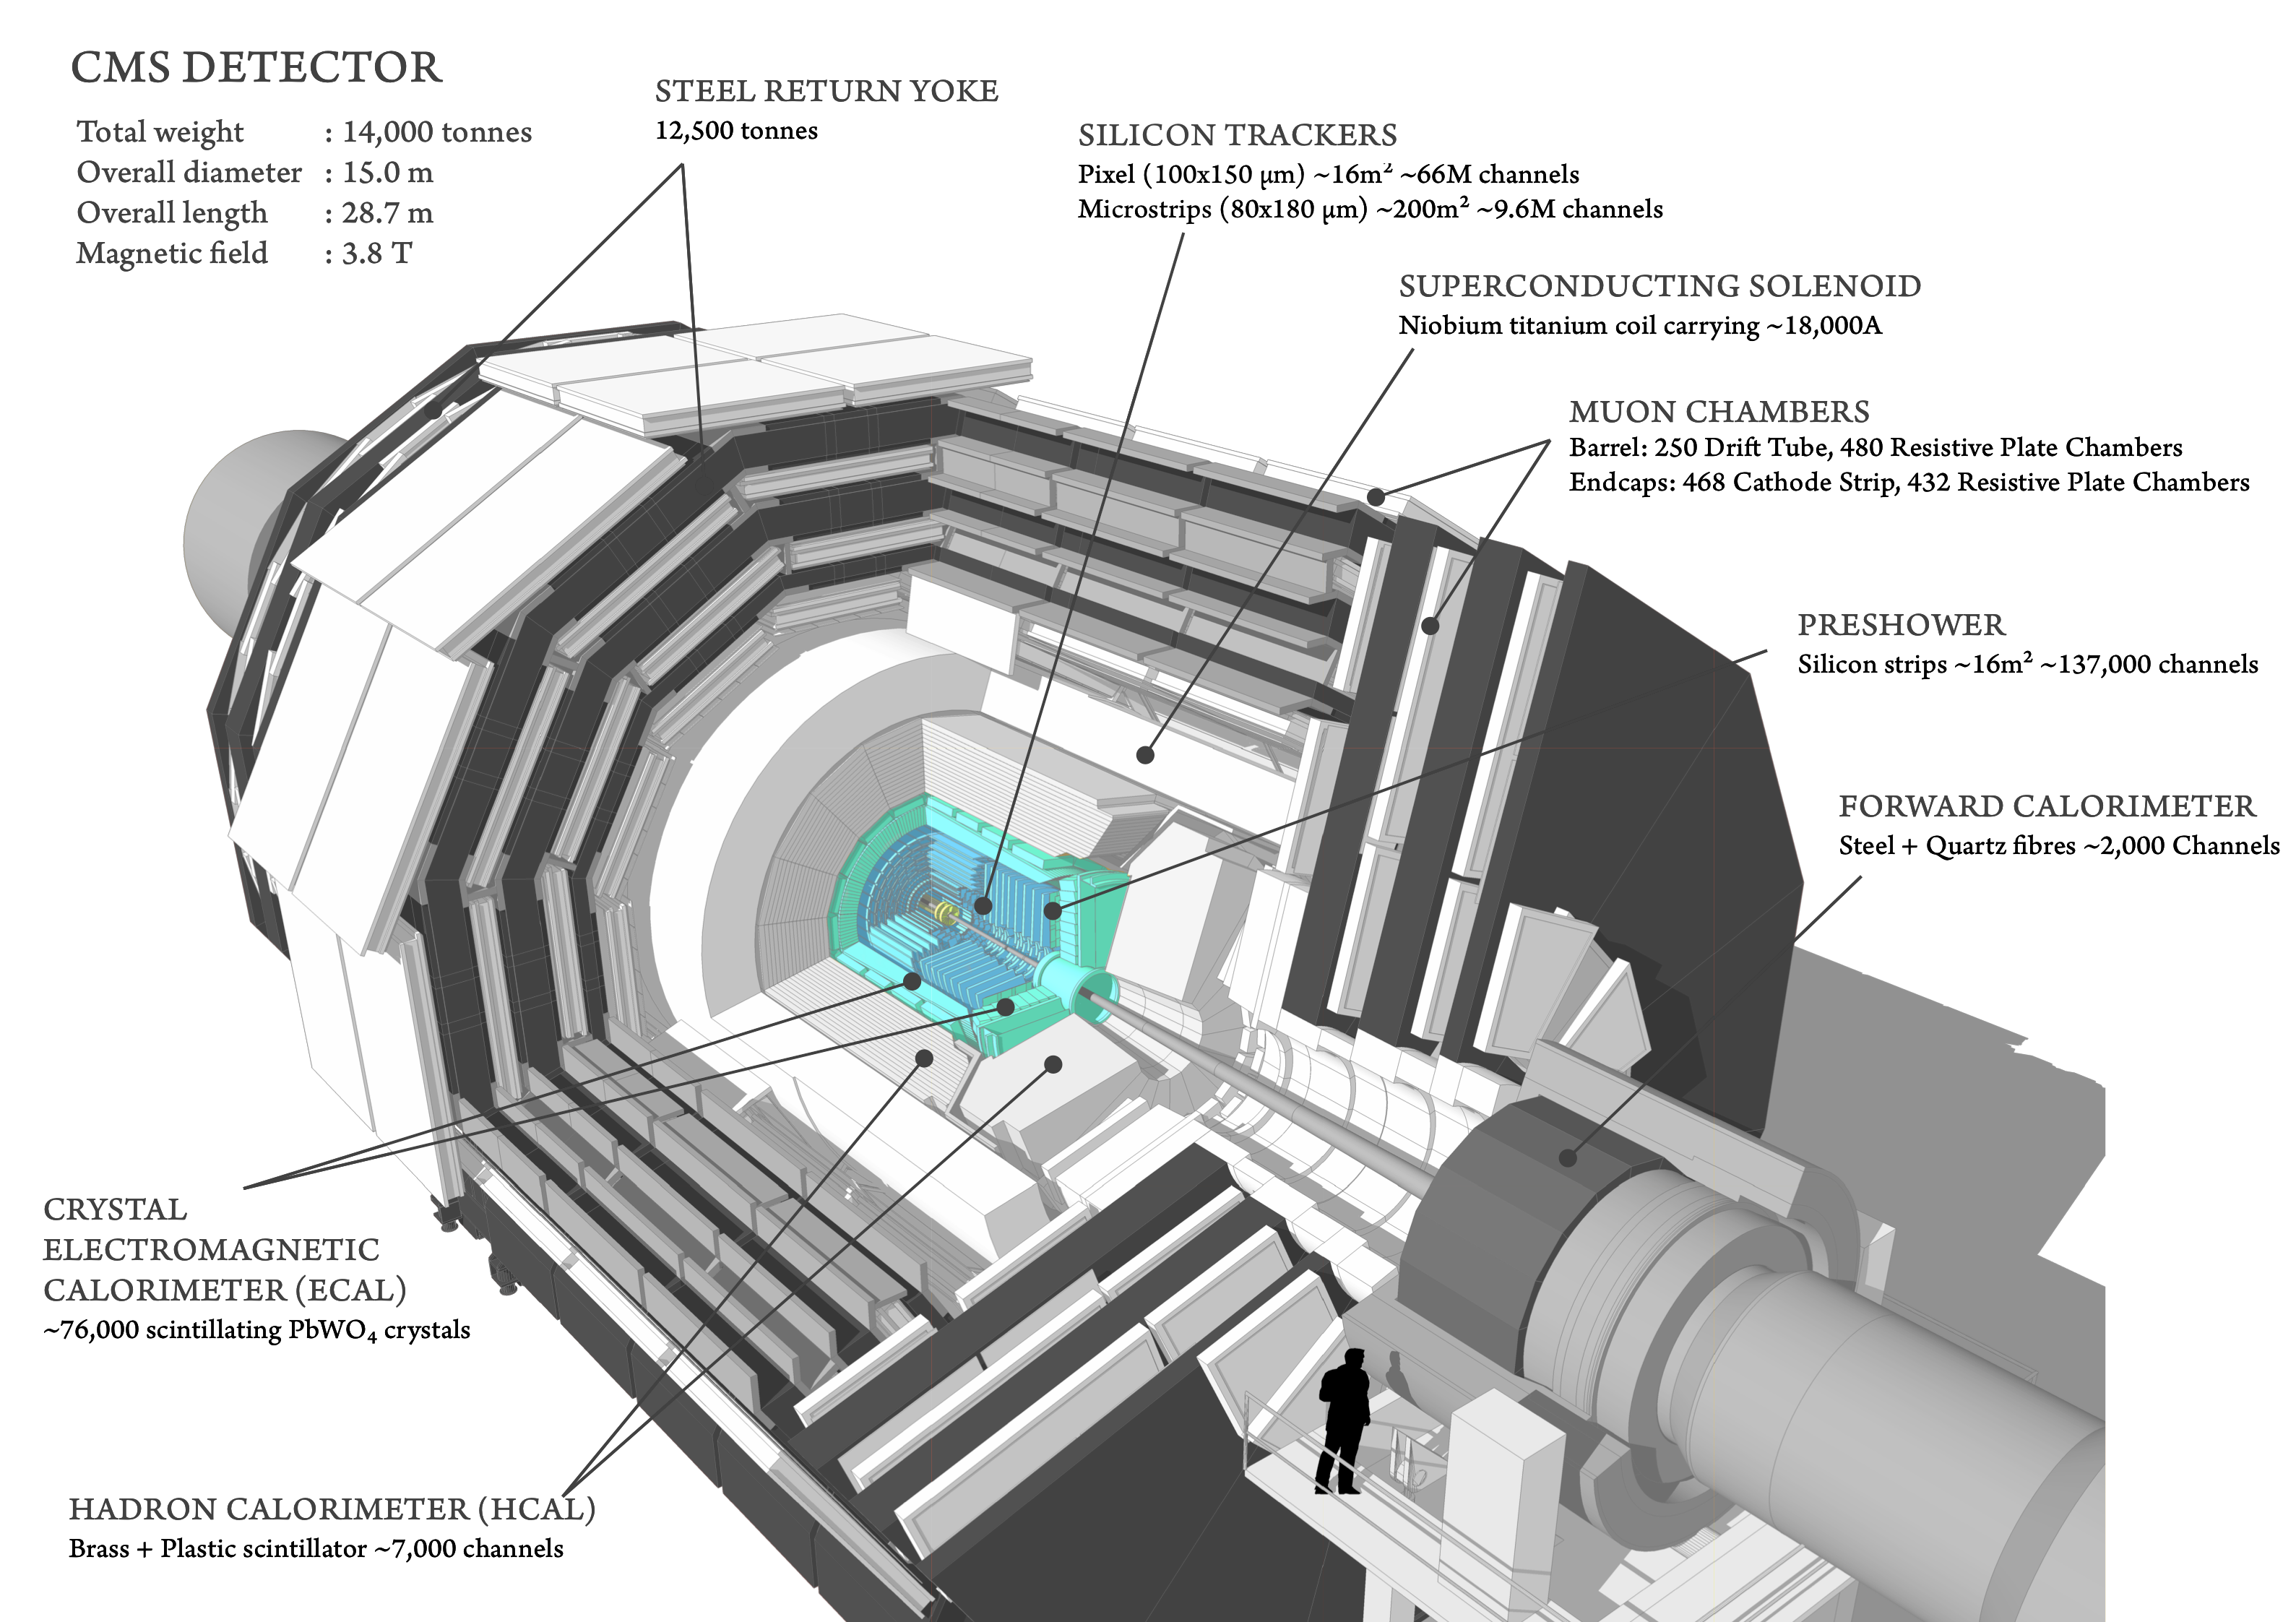
\includegraphics[width=0.95\textwidth]{cms_em.png}
	\end{center}}
		\only<4>{\begin{center}
		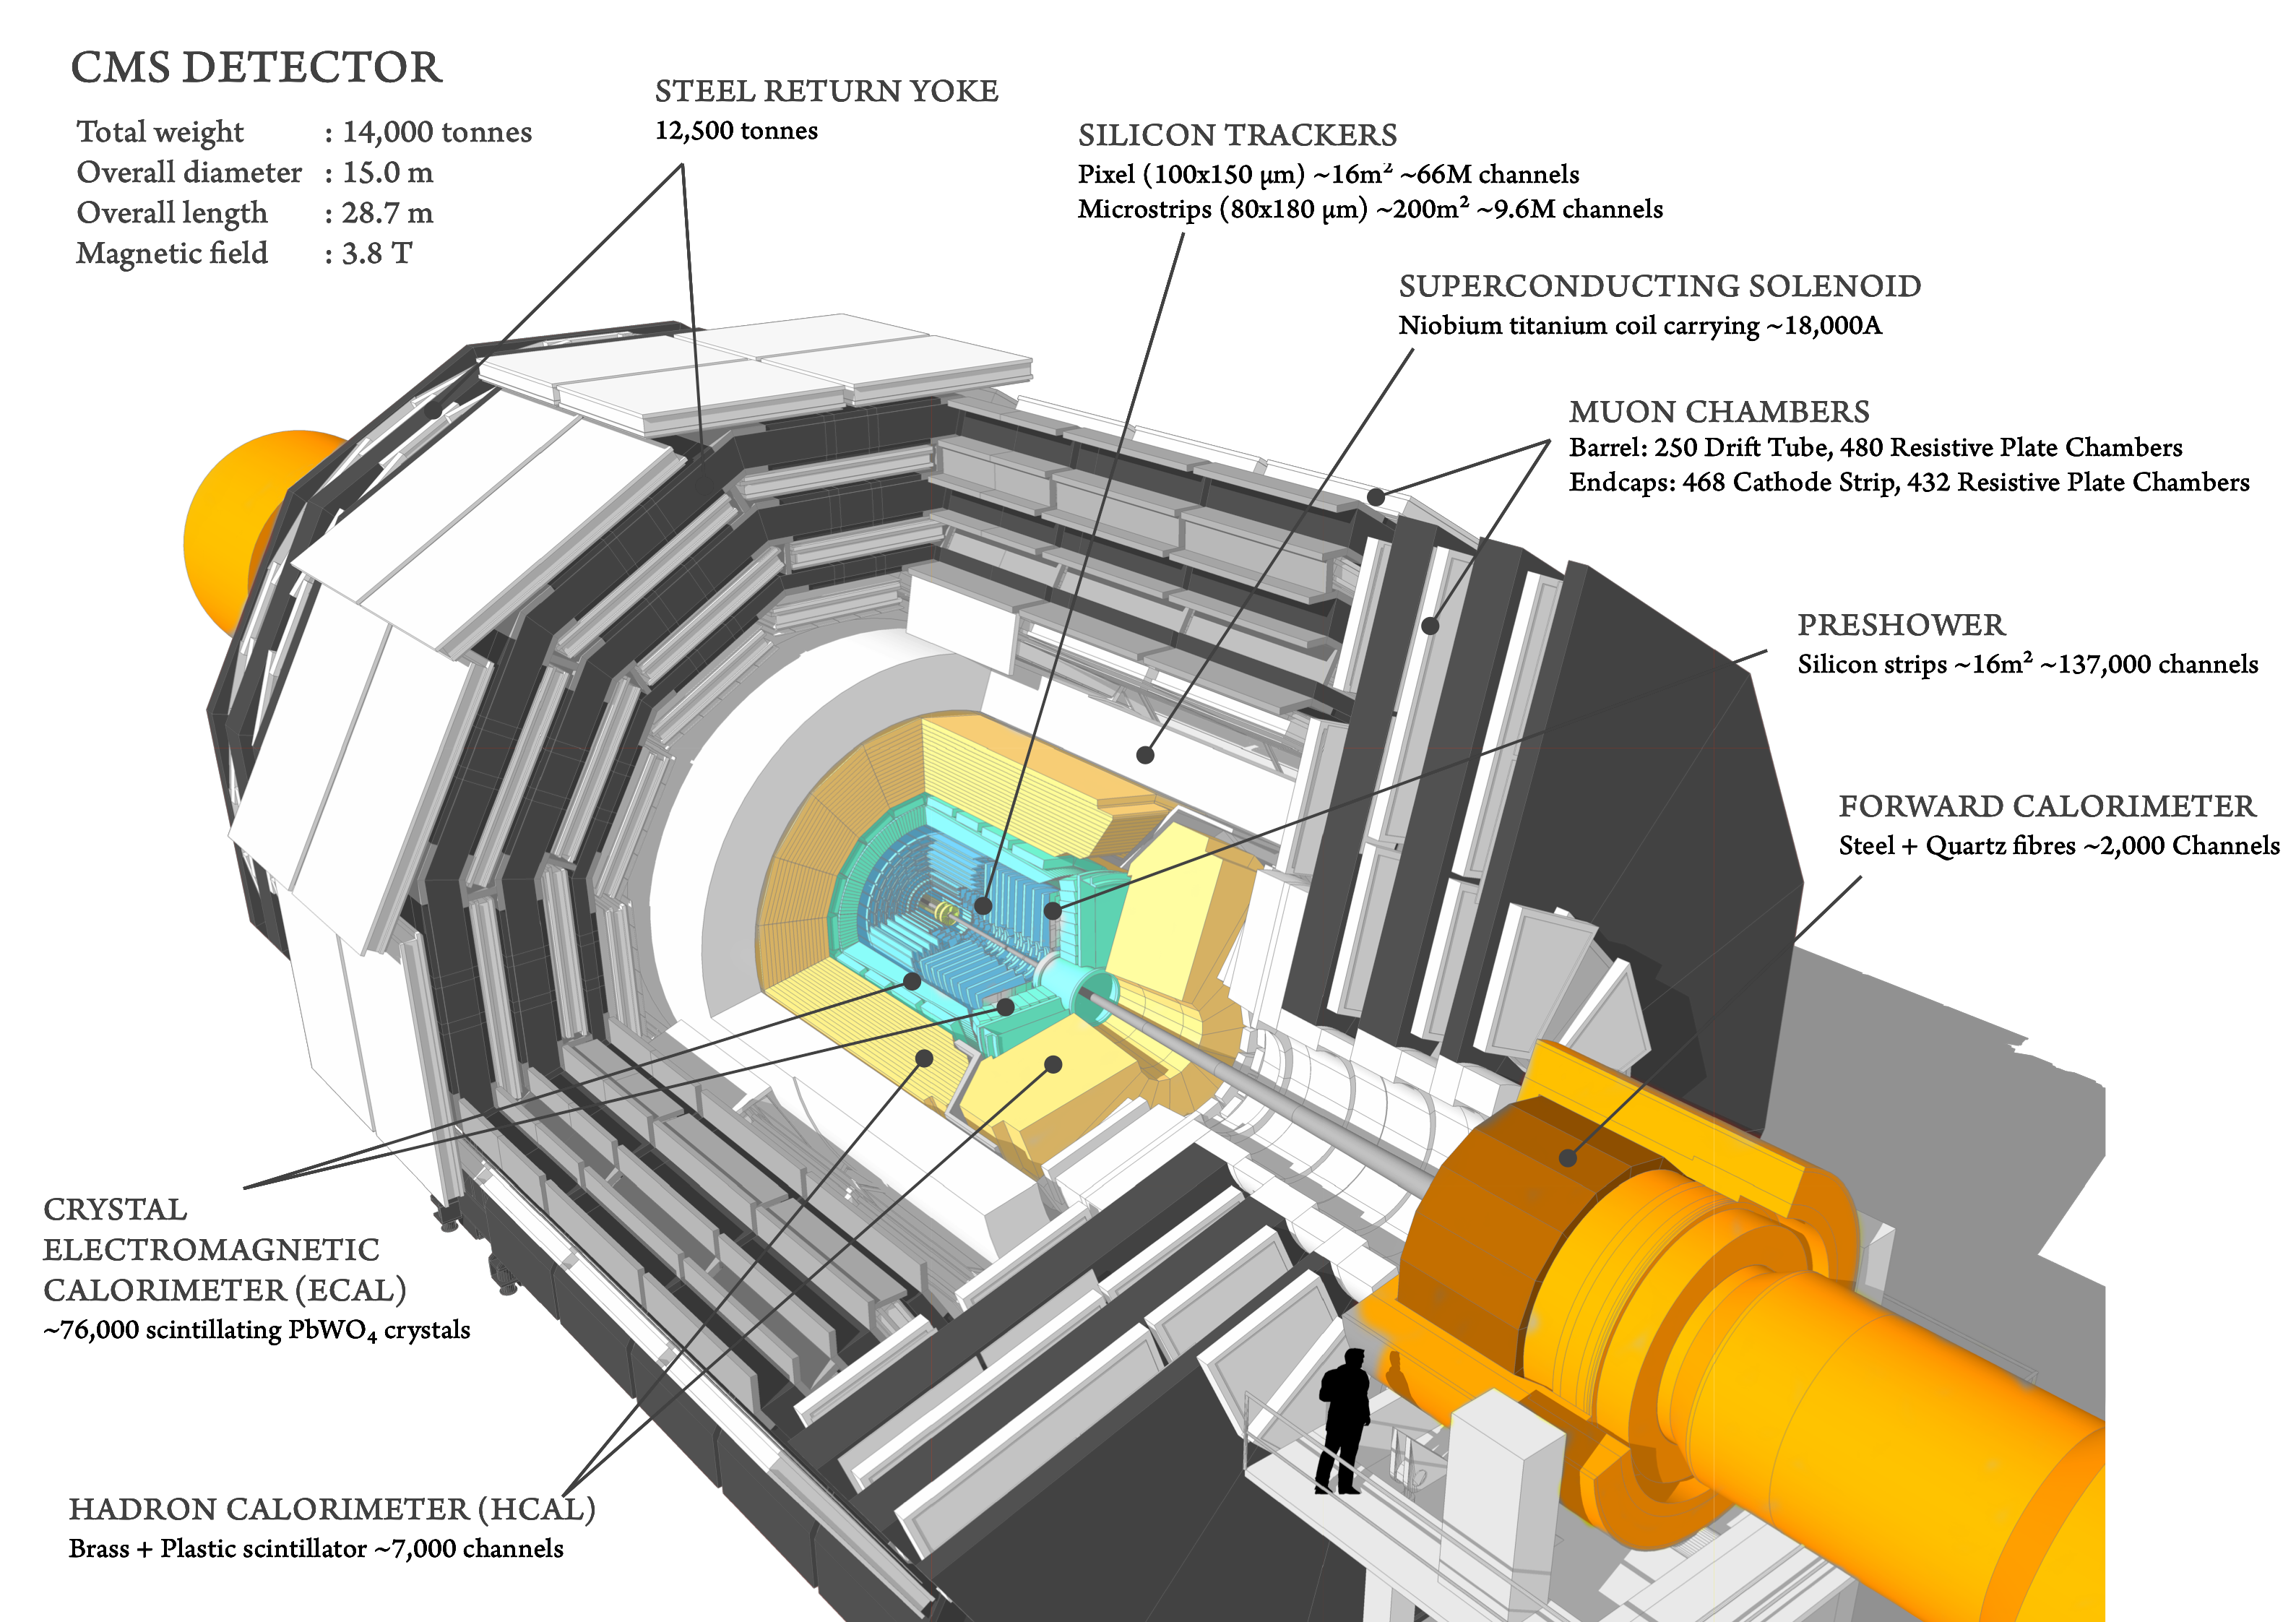
\includegraphics[width=0.95\textwidth]{cms_ha.png}
	\end{center}}
		\only<5>{\begin{center}
		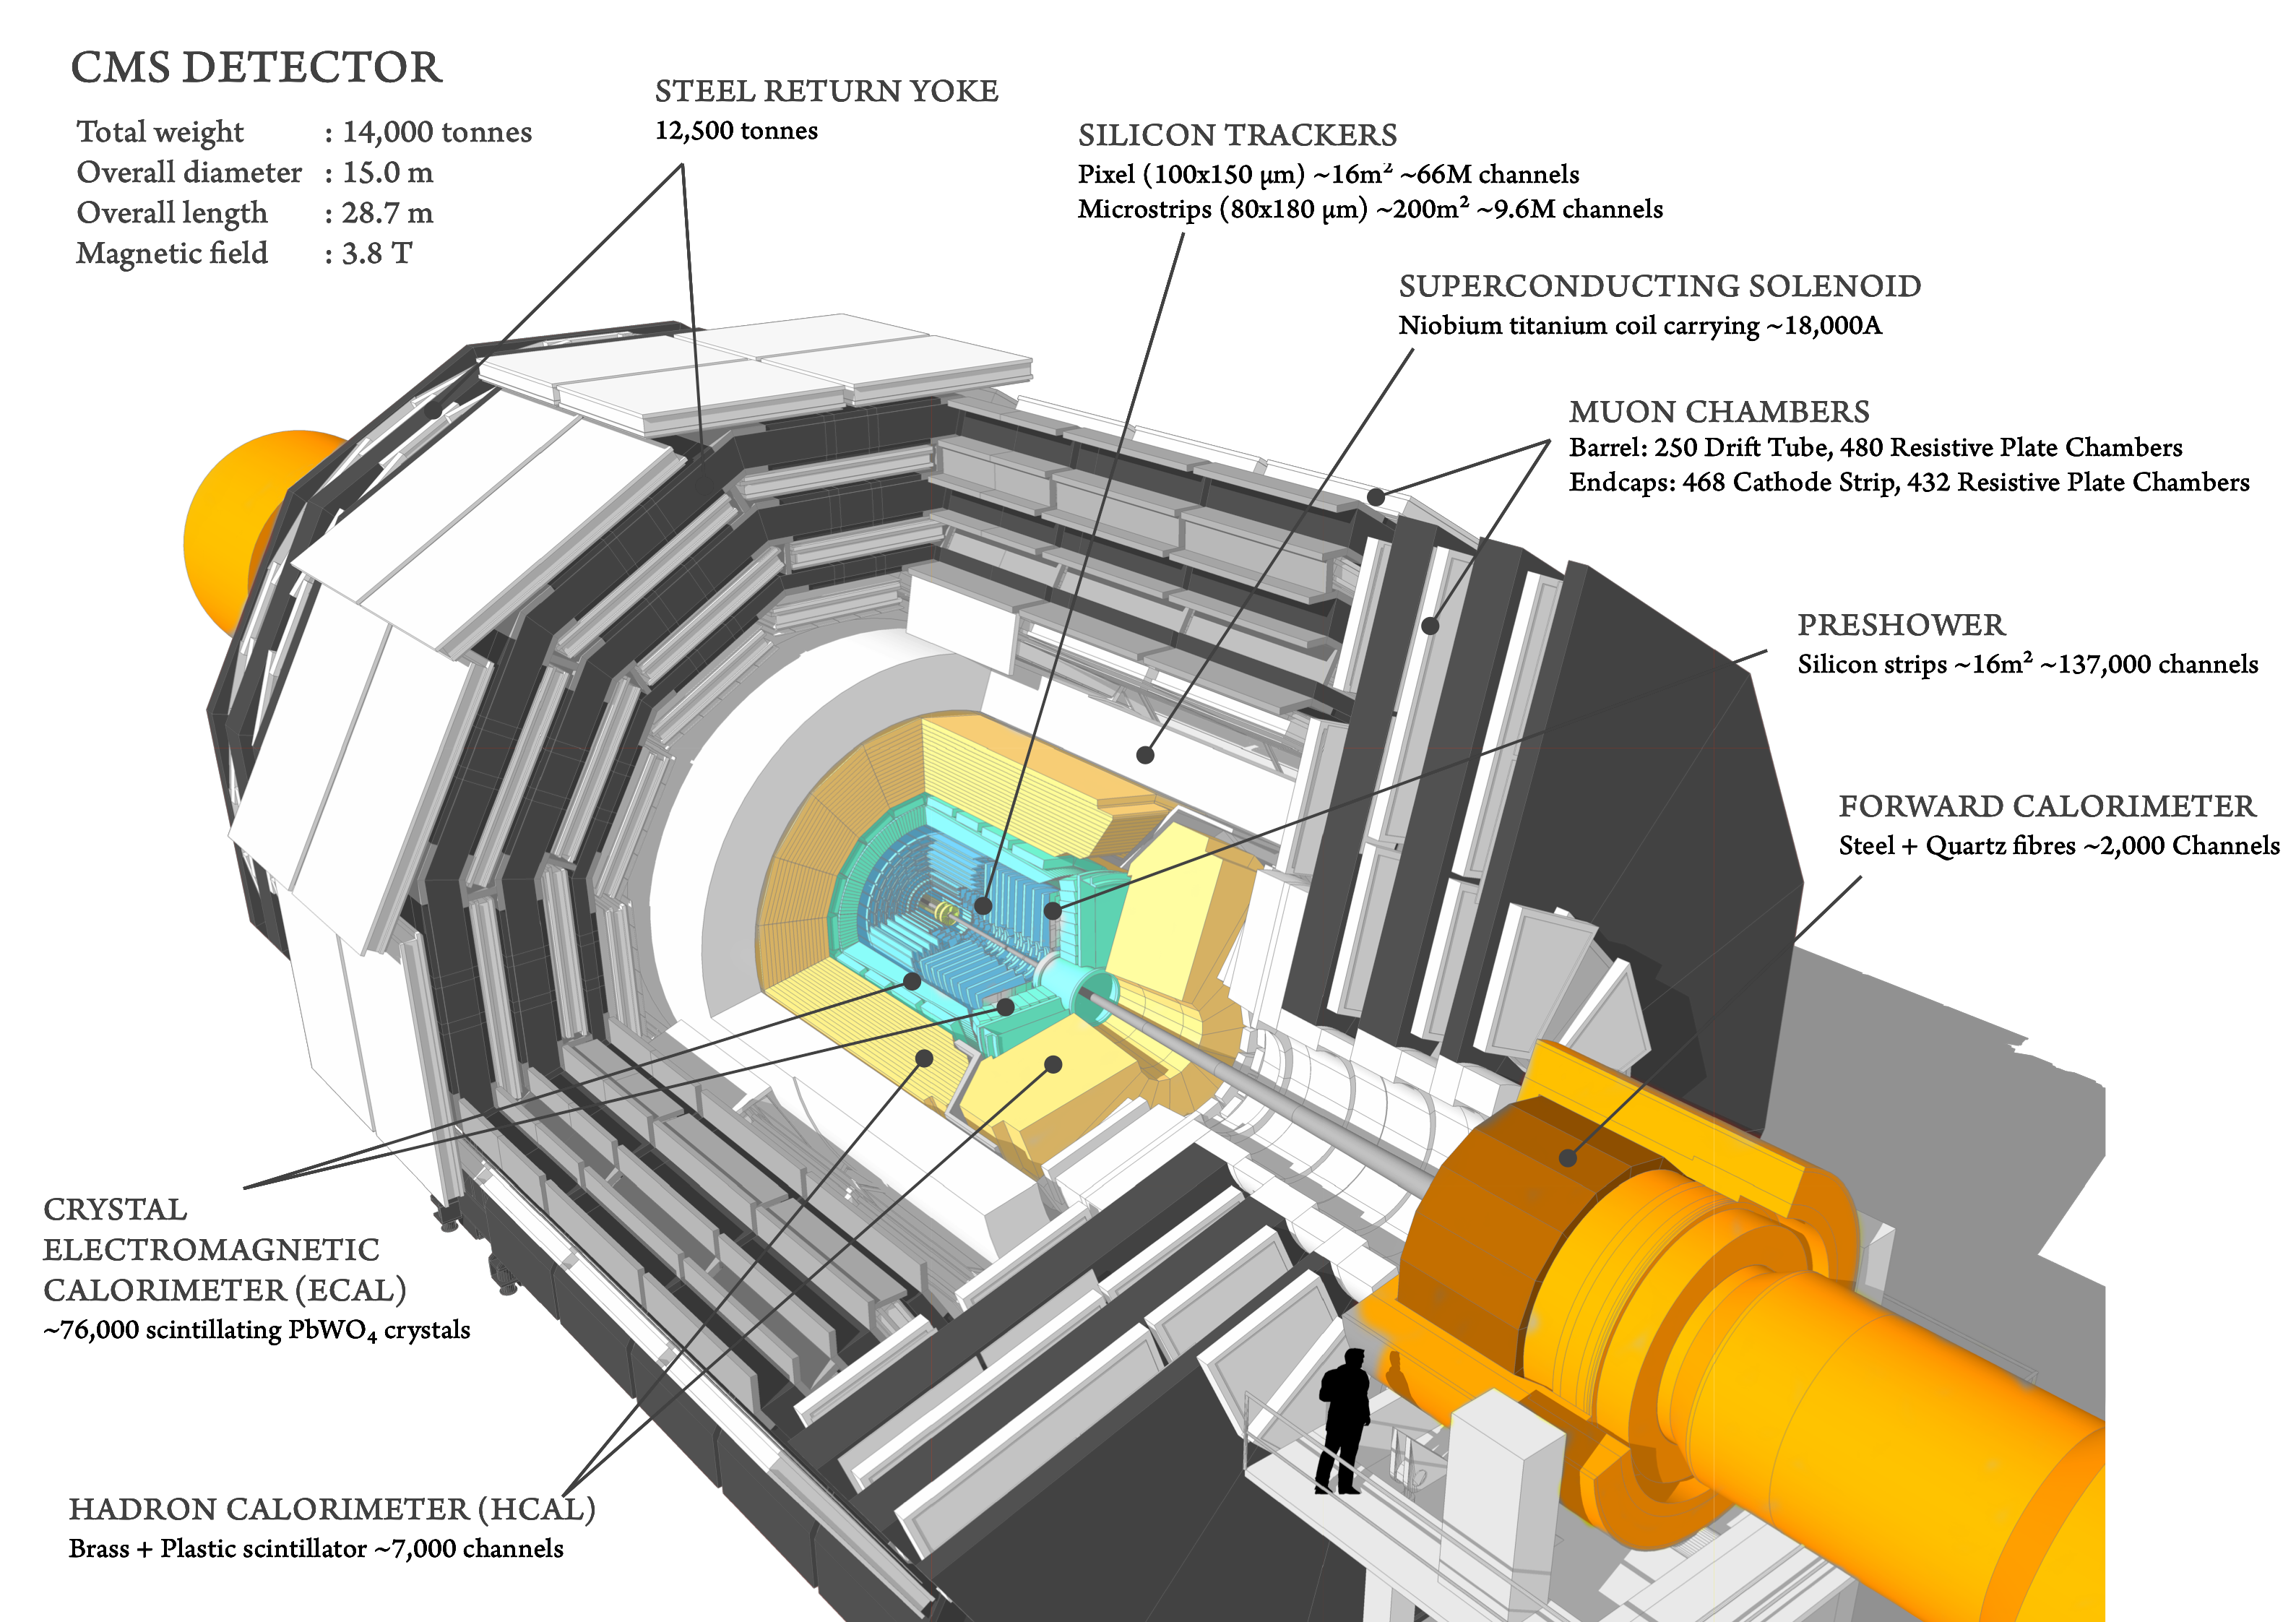
\includegraphics[width=0.95\textwidth]{cms_ha.png}
	\end{center}}
		\only<6>{\begin{center}
		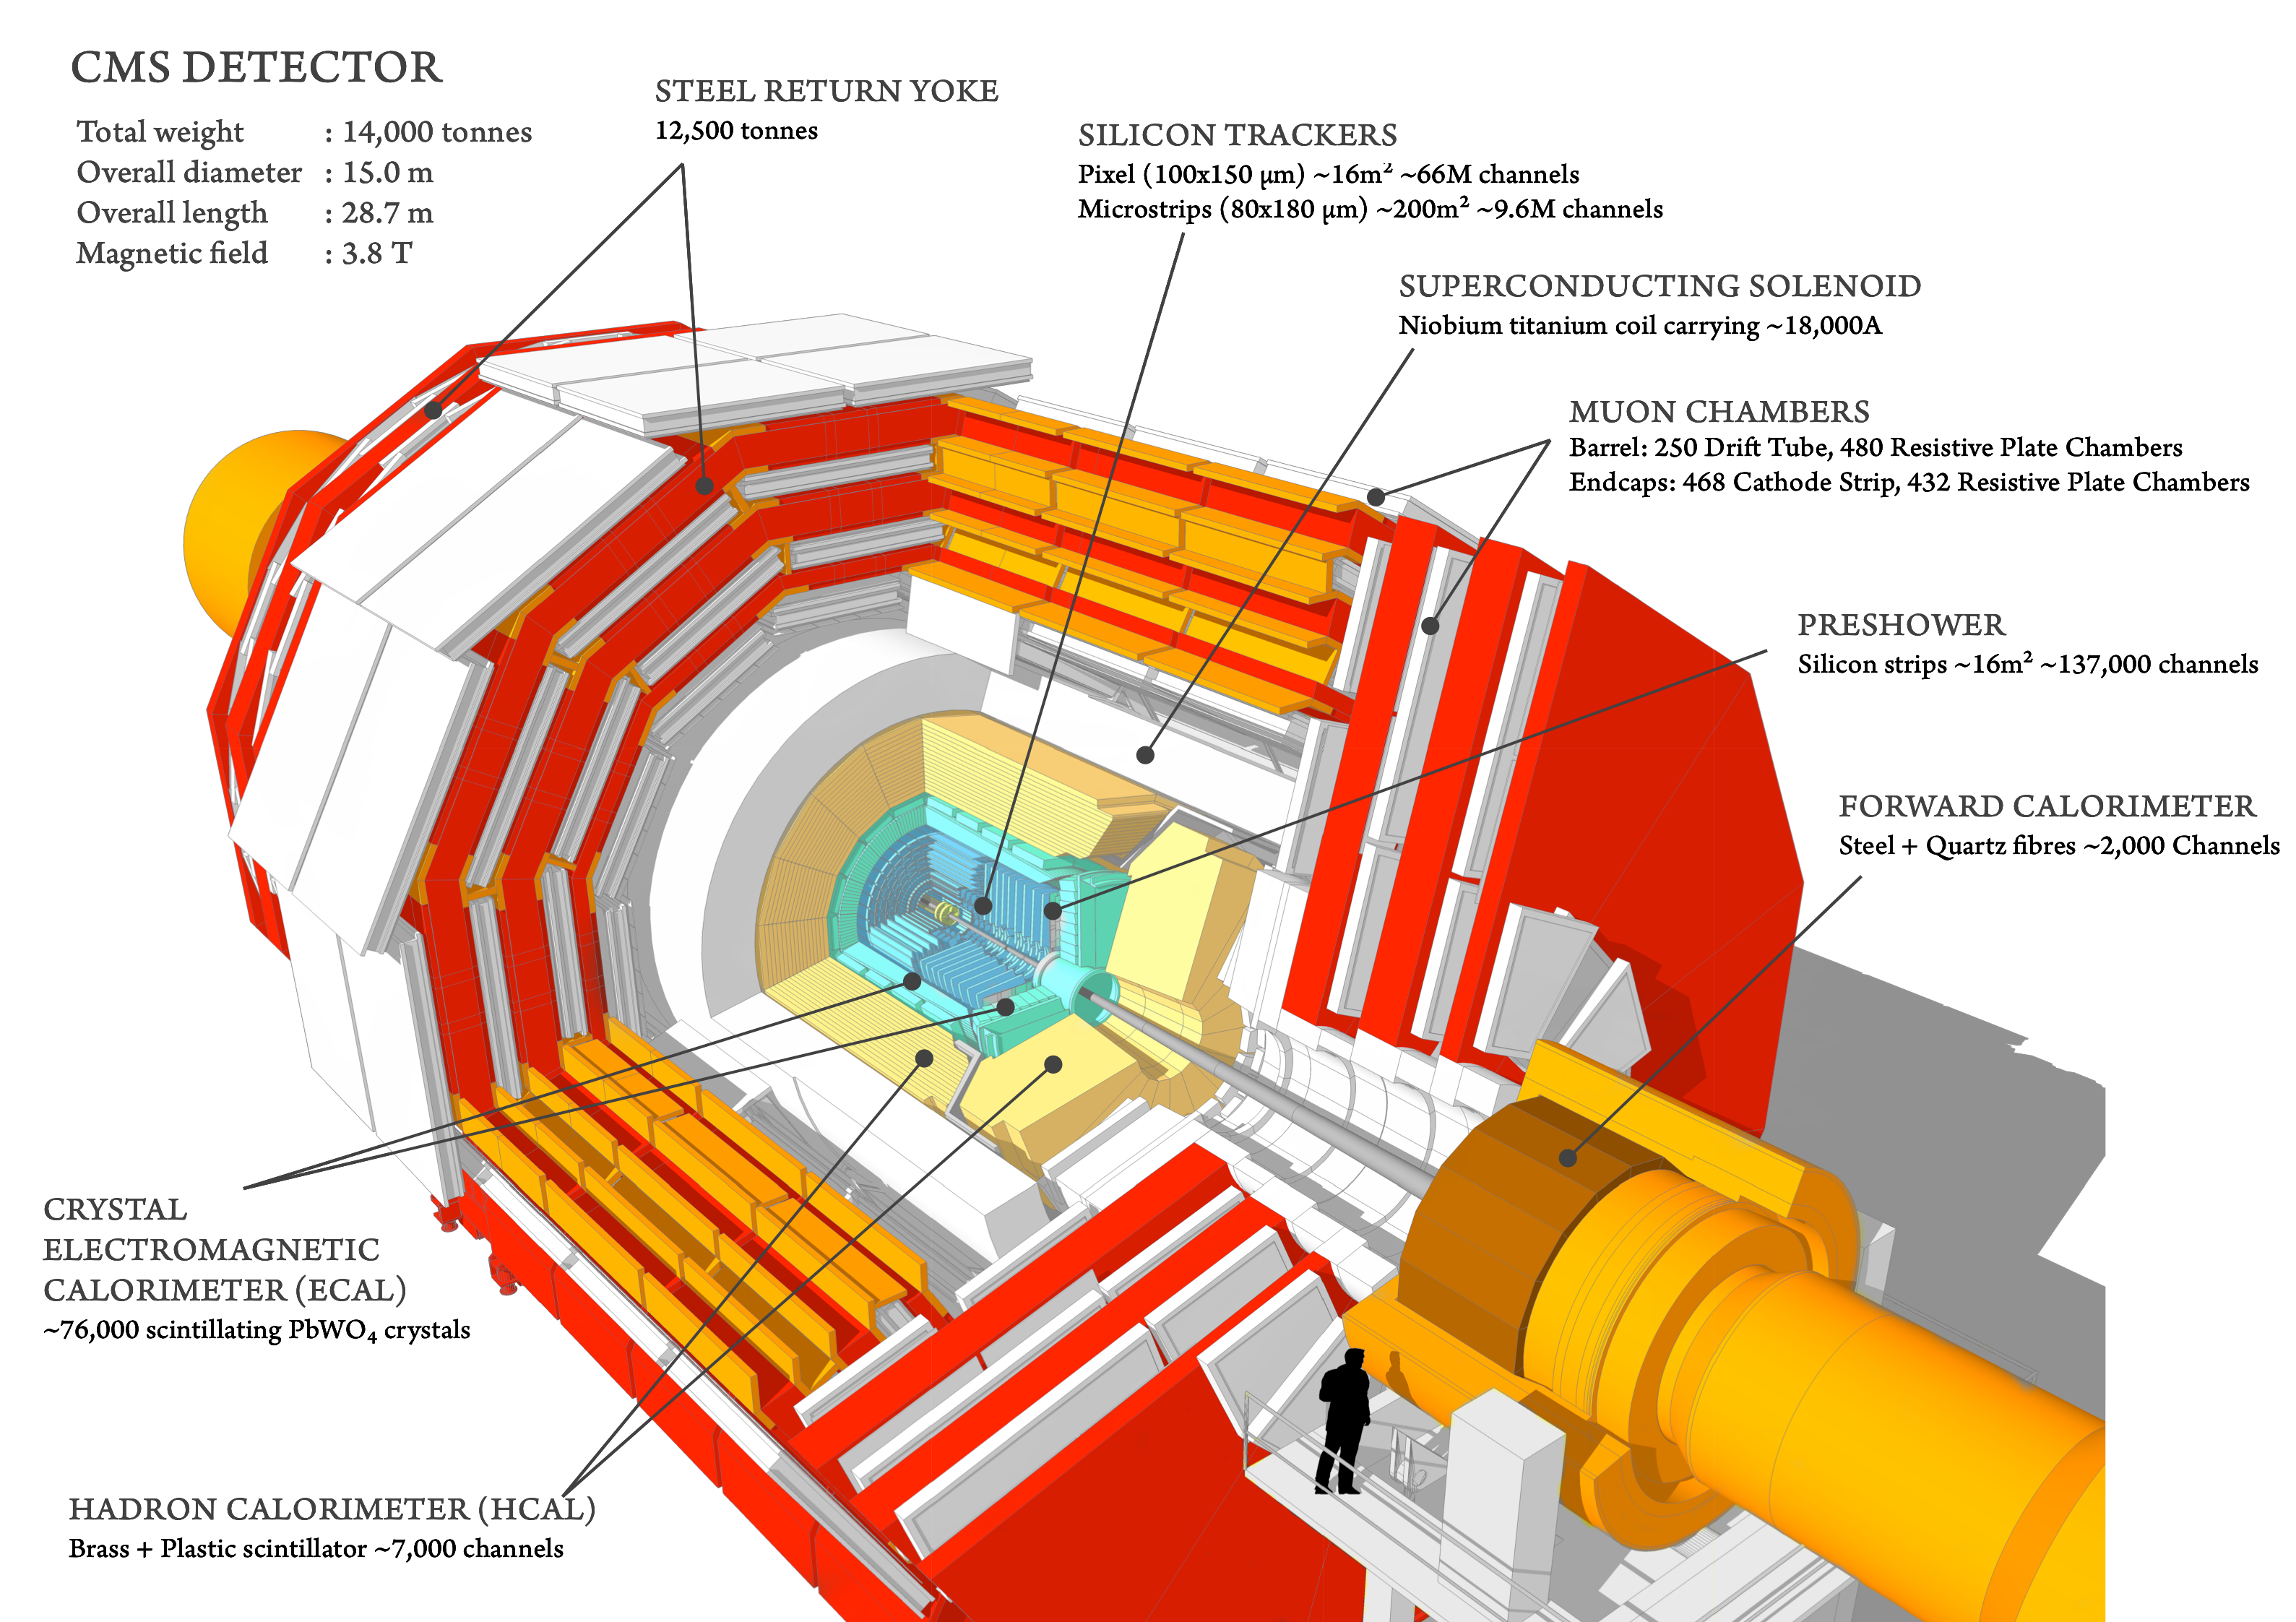
\includegraphics[width=0.95\textwidth]{cms_spectro.png}
	\end{center}}
	\end{block}
	\end{frame}
    \subsection{Le spectomètre à muons}
    \begin{frame}
    \begin{columns}
    	\column{.5\textwidth}
    	\begin{block}{\centering Chambres actuelles}
    		\begin{itemize}
    			\item \textit{Drift Tube} dans le tonneau
    			\item \textit{Cathode Strip Chamber} dans les bouchons
    			\item \textit{Resistive Plate Chamber}  dans les bouchons et le tonneau.
    		\end{itemize}
    	\end{block}
    \visible<2-4>{
          	\begin{block}{\centering Chambres pour la mise à niveau}
       	\begin{itemize}
       		\item <1-| alert@3> \textit{Gas Electron Multiplier}\,\tikz[na] \coordinate (gem);
       		\item <1-| alert@4> \textit{improved RPC}\,\tikz[na] \coordinate (irpc);
       	\end{itemize}
       \end{block}}
    	\column{.60\textwidth}
    	\begin{tikzpicture} 
    		\node [inner sep=0pt,above right]{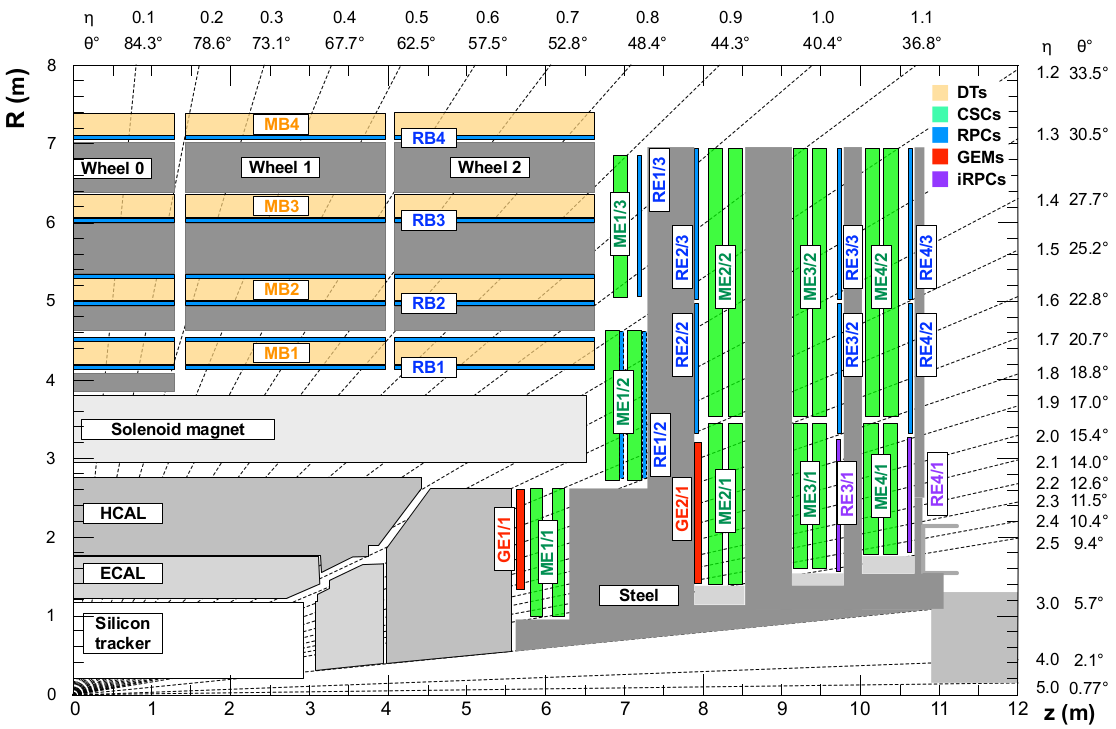
\includegraphics[width=1\textwidth]{endcap.png}};
    		\path (5.3,1.4) coordinate (irpc2);
    		\path (4.9,1.4) coordinate (irpc3);
    		\path (4.1,1.1) coordinate (gem2);
    		\path (3.0,1.1) coordinate (gem3);
    	\end{tikzpicture}
    \end{columns}
    \begin{tikzpicture}[overlay]
		\draw<3> [thin, red,opacity=.8, fill=red,fill opacity=0.3](gem2) circle (4pt);
		\path<3>[->,>=latex', red, shorten >=4pt, opacity=.6] (gem) edge  (gem2);
		\draw<3> [thin, red,opacity=.8, fill=red,fill opacity=0.3](gem3) circle (4pt);
		\path<3>[->,>=latex', red, shorten >=4pt, opacity=.6] (gem) edge  (gem3);
		\draw<4> [thin, red,opacity=.8, fill=red,fill opacity=0.3](irpc2) circle (4pt);
		\path<4>[->, >=latex', red, shorten >=4pt, opacity=.6] (irpc) edge  (irpc2);
		\draw<4> [thin, red,opacity=.8, fill=red,fill opacity=0.3](irpc3) circle (4pt);
		\path<4>[->, >=latex', red, shorten >=4pt, opacity=.6] (irpc) edge (irpc3);
	\end{tikzpicture}
	\end{frame}
	\section[RPC]{Les Resistive Plate Chambers (RPC)}
	\subsection{Description d'une RPC}
	\begin{frame}
	\begin{overlayarea}{0.99\textwidth}{8cm}
	\begin{block}{\centering Schéma typique d'une RPC}
		\begin{center}
		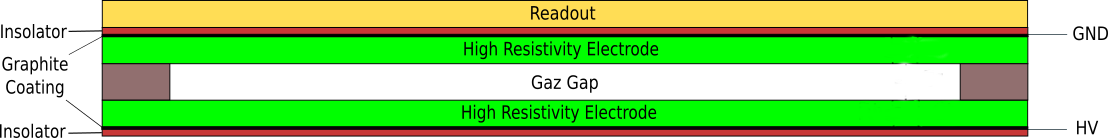
\includegraphics[width=1\linewidth]{scheme_first.png}
		\end{center}
	\end{block}
    \visible<2-5>{
	\begin{block}{\centering Le mode avalanche}
		\begin{overlayarea}{0.99\textwidth}{4cm}
		\begin{center}
		\only<2>{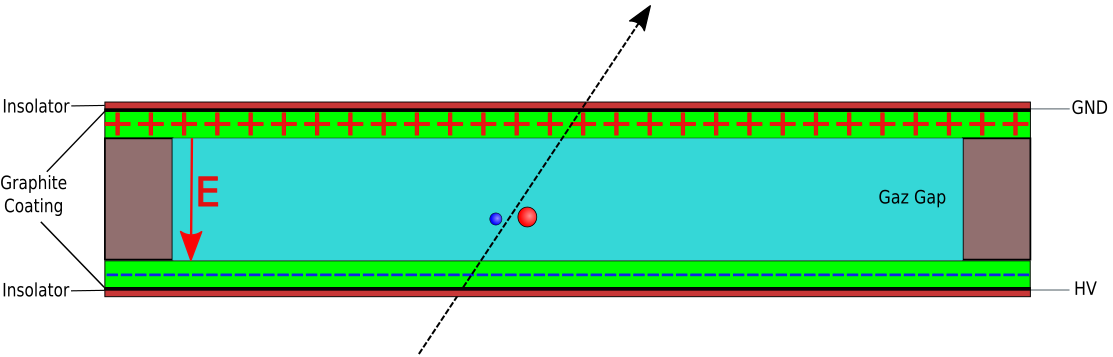
\includegraphics[width=1\linewidth]{avalanche-1.png}}
		\only<2>{\centering Ionisation primaire.}
		\only<3>{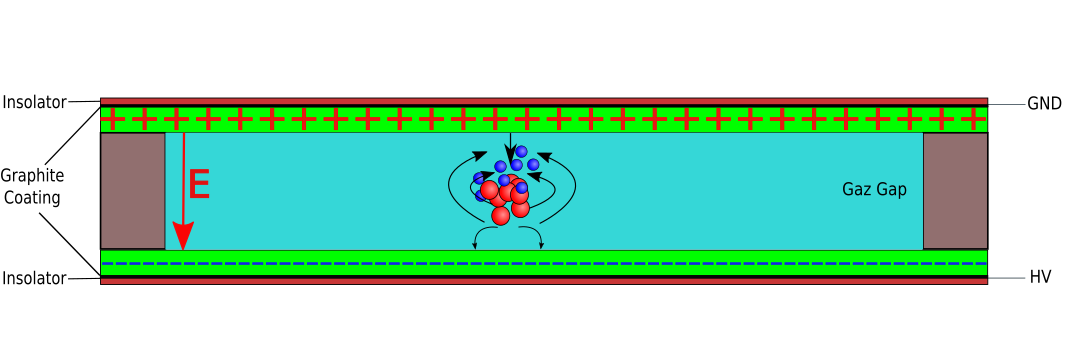
\includegraphics[width=1\linewidth]{avalanche-2.png}}
		\only<3>{\centering Ionisation secondaires. Création de l'avalanche.}
		\only<4>{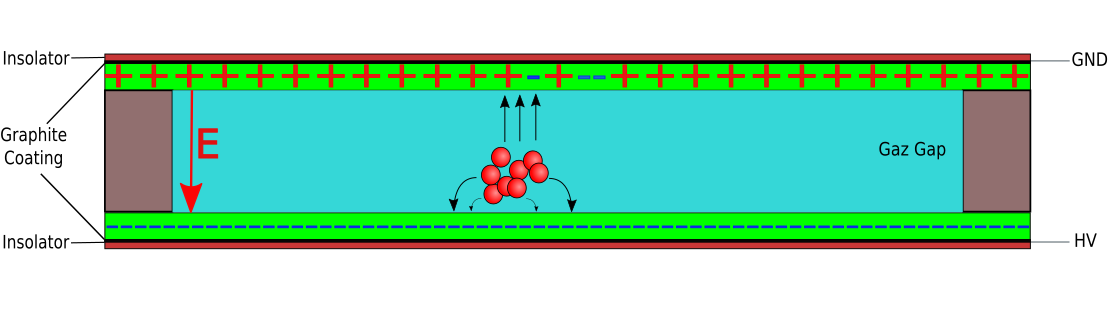
\includegraphics[width=1\linewidth]{avalanche-3.png}}
		\only<4>{\centering Les électrons atteignent l'anode, les ions sont beaucoup plus lents.}
		\only<5>{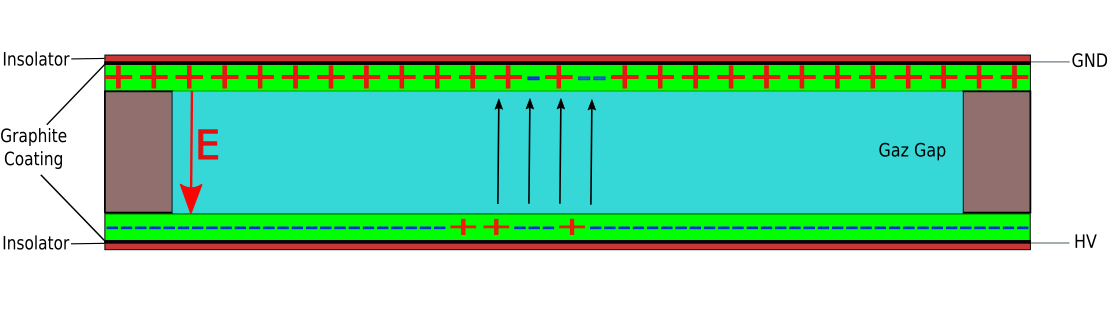
\includegraphics[width=1\linewidth]{avalanche-4.png}}
		\only<5>{\centering Les charges sur les électrodes induisent un temps mort.}
		\end{center}
		\end{overlayarea}
	\end{block}}
    \end{overlayarea}
	\end{frame}	
    \subsection{Les RPC dans les bouchons de CMS}
    \begin{frame}
    \begin{block}{\centering Les détecteurs}
    \begin{center}
   	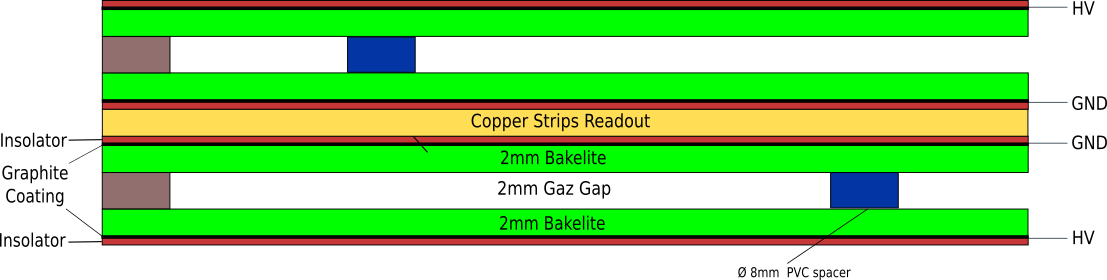
\includegraphics[width=0.6\linewidth]{CMSRPC.png}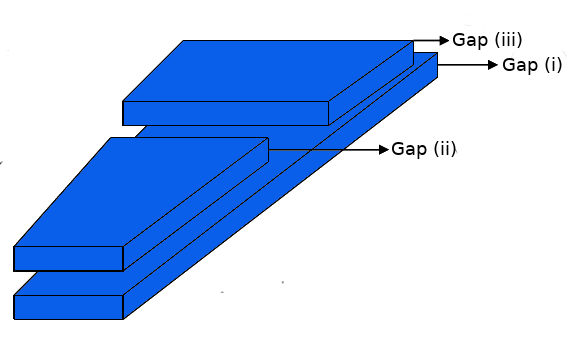
\includegraphics[width=0.4\linewidth]{gaps.png}
   	\end{center}
    	\begin{itemize}
    		\item Chambre \textit{double gaps} de \SI{2}{\milli\meter}
    		\item Électrodes en Bakélite ($\rho=1-6\times10^{10}$\si{\ohm\centi\meter})
    		\item Gas gap de \SI{2}{\milli\meter}
    	\end{itemize}
    \end{block}
	\begin{block}{\centering Mélange gazeux}
			\begin{itemize}
				\item 95.2\% de Tétrafluoroéthane \chemform{C_2H_2F_4} (R-134a).
				\item \num{4.5}\% d'isobutane \chemform{iso-C_4H_{10}}, absorbeur de photons UV. 
				\item \num{0.3}\% d'hexafluorure de soufre \chemform{SF_6}, capture l'excès d'électrons.
			\end{itemize}
	\end{block}
	\end{frame}
	\subsection{Les improved Resistive Plate Chambers}
	\begin{frame}
	Les RPC actuelles sont incapables de supporter le flux de particules présent dans les zones RE3/1 et RE4/1
	\begin{block}{\centering improved Resistive Plate Chambers}
	\begin{itemize}
		\item Résister au flux de particules ($\sim$\SI{700}{\hertz\per\square\centi\meter}),
		\item (\SI{2}{\kilo\hertz\per\square\centi\meter}) en prenant en compte un facteur 3 de sécurité
	\end{itemize}
	\end{block}
	
	\begin{block}{\centering Possibilités}
		\begin{itemize}
		\item Réduire l'épaisseur $d$ des électrodes $\rightarrow$ Nouvelles chambres Bakélite
		\item Réduire la charge $q$ créée par l'avalanche $\rightarrow$ Réduire l'épaisseur de gas.
		\item {\only<2>{\color{red}}Réduire la résistivité des électrodes $\rightarrow$ \textit{Low Resistivity Glass}}
	\end{itemize}
	\end{block}
	\end{frame}
	\section{Électrodes de verre de basse résistivité}
	\subsection{Les verres de basse résistivité}
	\begin{frame}
	\begin{columns}
		\column{.65\textwidth}
		\begin{block}{\centering Caractéristiques}
			\begin{itemize}
				\item {\color{Green}Résistivité volumique} : {\color{Green}\SI{e10}{\ohm.\centi\meter}}
				\item {\color{Green}Épaisseur} : {\color{Green}\SIrange{0.5}{2}{\milli\meter}}
				\item {\color{Green}Uniformité de l'épaisseur} : {\color{Green}\SI{0.02}{\milli\meter}}
				\item {\color{Green}Rugosité} : {\color{Green}$<$\SI{10}{\nano\meter}}
				\item {\color{Green}Comportement ohmique} : {\color{Green} stable (\SI{1}{\coulomb})}
				\item {\color{red}Dimension maximale} : {\color{red}\SI{32}{\centi\meter}$\times$\SI{30}{\centi\meter}}
			\end{itemize}
		\end{block}
		\column{.3\textwidth}
		\begin{center}
		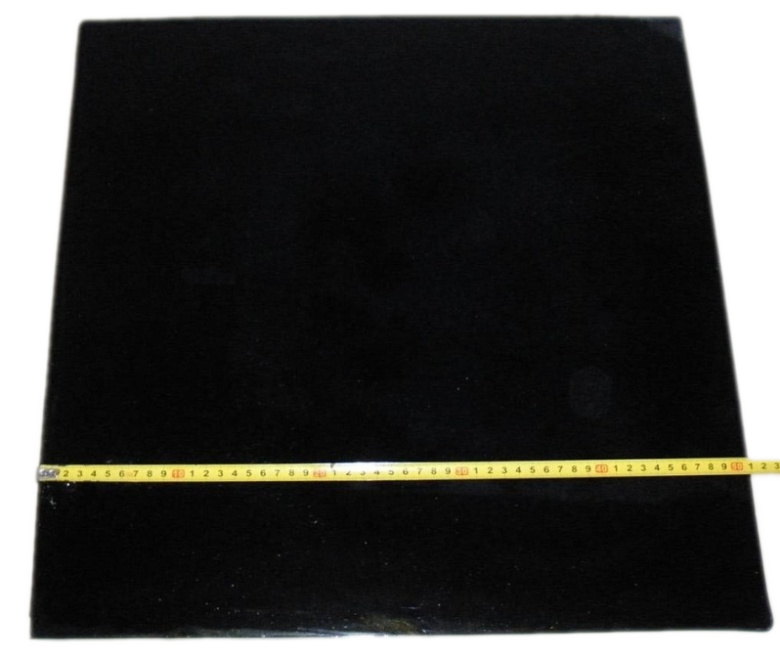
\includegraphics[width=0.7\textwidth]{verre.png}
		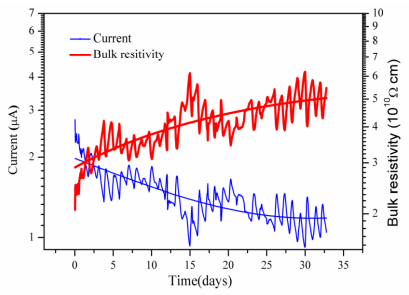
\includegraphics[width=1.1\textwidth]{resi.png}
		\end{center}
	\end{columns}
	\begin{block}{\centering Chambre single gap}
		\begin{itemize}
			\item Épaisseur des électrodes \SI{1}{\milli\meter}
			\item Épaisseur du gaz \SI{1.2}{\milli\meter}
			\begin{center}
			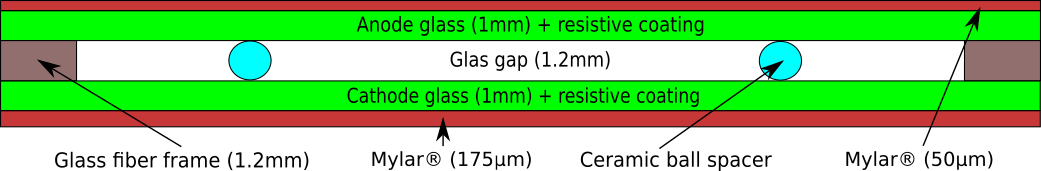
\includegraphics[width=0.8\textwidth]{gap.png}
			\end{center}
		\end{itemize}
	\end{block}
\end{frame}
	\subsection{L'électronique à base de HARDROC}
	\begin{frame}
	\begin{block}{\centering Le HARDROC}
		\begin{columns}
			\column{.6\textwidth}
		\begin{itemize}
			\item Développé par le groupe OMEGA
			\item 64 canaux
			\item 3 seuils
			\item Gamme dynamique : \SI{10}{\femto\coulomb}-\SI{15}{\pico\coulomb} 
		\end{itemize}
		\column{.4\textwidth}
		\begin{center}
		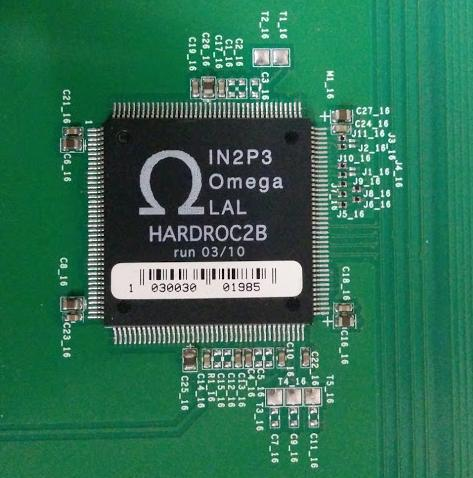
\includegraphics[width=0.5\textwidth]{hardroc2.jpg}
		\end{center}
	\end{columns}
	\end{block}
	\begin{columns}
		\column{.5\textwidth}
		\begin{block}{\centering PCB à pads}
			\begin{center}
			Pads de \SI{1}{\centi\meter}$\times$\SI{1}{\centi\meter}
			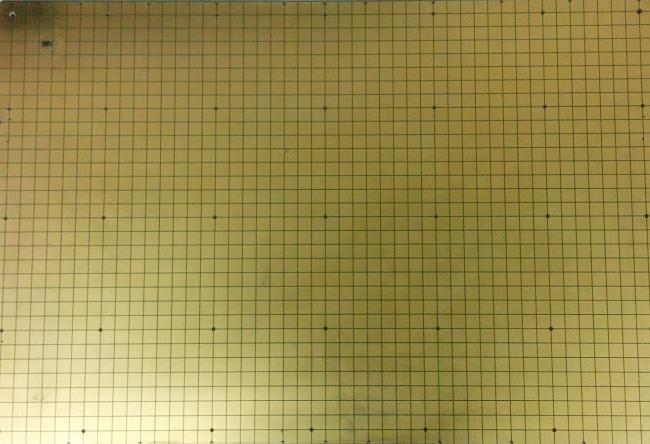
\includegraphics[width=0.5\textwidth]{cellules.jpg}
		\end{center}
		\end{block}
		\column{.5\textwidth}
	    \begin{block}{\centering PCB à strip}
	    	\begin{center}
	    		128 strips de \SI{2}{\milli\meter} de largeur des 2 côtés du PCB. 
	        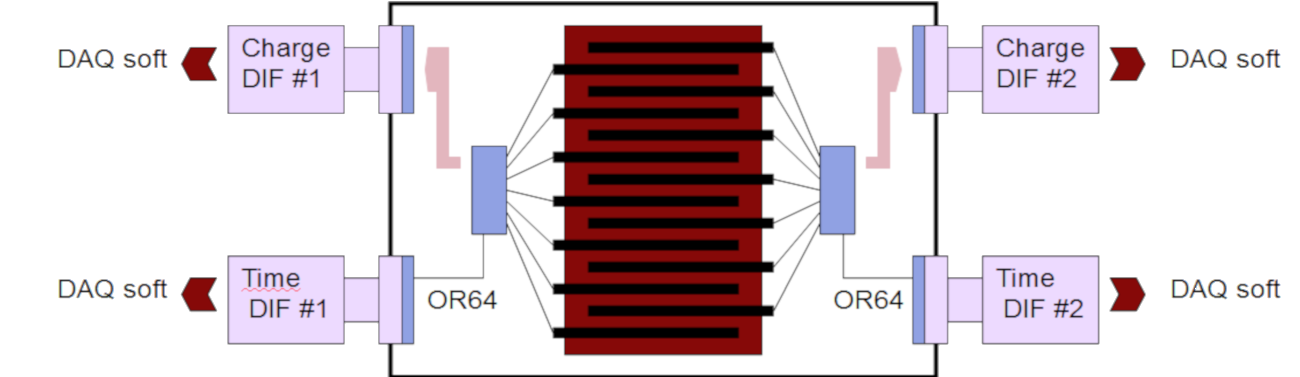
\includegraphics[width=1\textwidth]{SchemePS.png}
	    \end{center}
	    \end{block}
	\end{columns}
	\end{frame}
    \subsection{Caractérisation des Glass Resistive Plate Chambers}
    \begin{frame}
    \begin{block}{\centering Éléments importants pour la caractérisation d'une chambre}
    	\begin{itemize}
    		\item L'efficacité de détection :  le rapport entre le nombre de particules ayant réellement été détectées et le nombre total de particules ayant traversé la chambre. 
    		\item La multiplicité (\textit{Cluster Size}) : Le nombre de pads ou strips touchés lorsqu’une particule traverse la chambre.
    		\item Le bruit électronique : La fréquence de détection par l’électronique, d’un signal considéré comme non physique. 
    		\item Sensibilité au bruit de fond (photons, neutrons, \ldots)
    		\item Le vieillissement : Évolution des caractéristiques de la chambre en fonction du temps.
    	\end{itemize}
    \end{block}
	\end{frame}
	\subsection{Programme d'analyse des données}
	\begin{frame}
	\begin{block}{\centering Méthode par reconstruction de traces}
		\begin{itemize}
			\item Mise en forme des données brute
			\item Prise en compte de la géométrie du détecteur (XML)
			\item Présélection des candidats muon (agrégation en temps) :
				\begin{itemize}
					\item $>$3 Hits dans un coup d'horloge.
					\item Sélection d'une fenêtre $t_{fen}=\pm3$ 
				\end{itemize}
			\item Barycentre des hits dans chaque chambre
			\item Création d'un candidat trace par minimisation du $\chi^2$
			\item Sélection des hits dans la chambre étudiée qui sont a $\pm3$ pads (strips) de la trace .
		\end{itemize}
		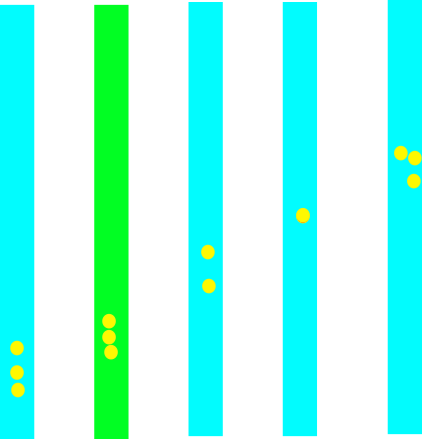
\includegraphics[width=0.25\textwidth]{1.png}
		\hfill
		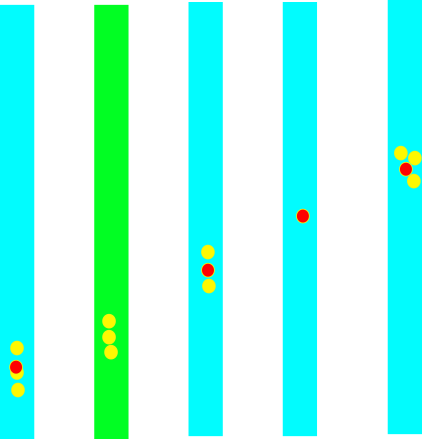
\includegraphics[width=0.25\textwidth]{2.png}
		\hfill
		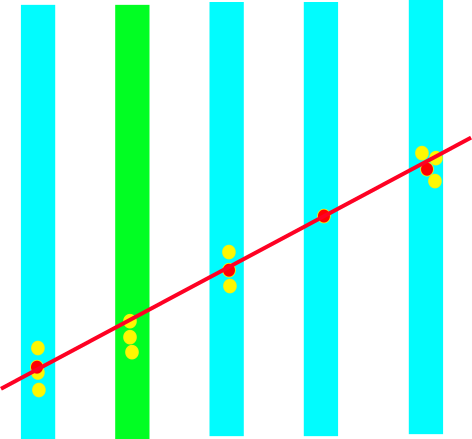
\includegraphics[width=0.285\textwidth]{3.png}
	\end{block}
	\end{frame}
	\subsection{Programme d'analyse des données}
	\begin{frame}
		\begin{columns}
			\column{.6\textwidth}
			\begin{block}{\centering Test du programme d'analyse}
				Simulation GEANT4 de SDHCAL développée à l'IPNL 
				\begin{itemize}
					\item Calcul de la longueur des segments contenus dans le volume de gaz correspondant à un pads $C_{0}$
					\item Application d'une carte d'efficacité 
					\item Sélection de la charge induite pour chaque segment en utilisant une Polya
					$P(q)=\left[\frac{q}{\bar{q}}(1+\theta)\right]^\theta\exp^{-\left[\frac{q}{\bar{q}}(1+\theta)\right]}$
					\item Correction de la charge en fonction de l'angle incident 
					\item Répartition des charges sur les cellules voisines se trouvant à une distance inférieur à $R_{max}$ de $C_0$
					\item Application des seuils électronique.
				\end{itemize}
			\end{block}
			\column{.5\textwidth}
			\begin{center}
			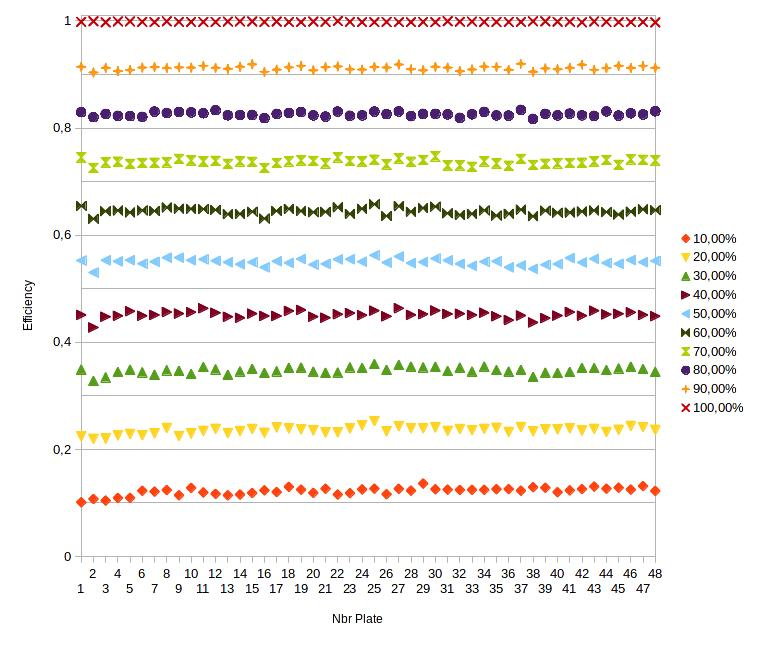
\includegraphics[width=1\textwidth]{effisimul.jpg}
			\end{center}
		\end{columns}
	\end{frame}
    \subsection{Test en faisceaux au PS (Zone Est) en juin 2014}
    \begin{frame}
    	\begin{columns}
    		\column{.55\textwidth}
    		\begin{block}{\centering Chambres}
    			\begin{itemize}
    				\item 8 chambres
    				\item 5 "float glass", 3 "Basse Résistivité"
    				\begin{center}
    				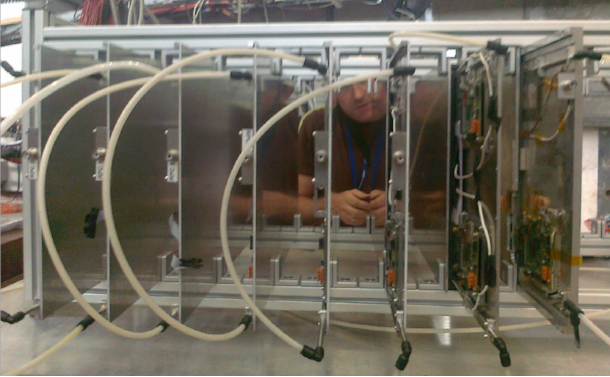
\includegraphics[width=0.65\textwidth]{TelescopePS.png}
    				\end{center}
    				\item Électronique HARDROC 
    				\item 7 à Pads, 1 à strips (Double gaps)
    				\begin{center}
    				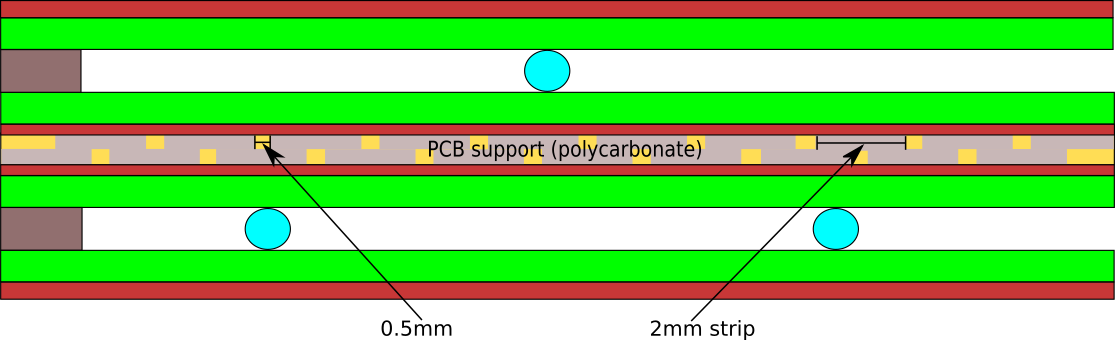
\includegraphics[width=0.8\textwidth]{DoubleGap.png}
    				\end{center}
    			\end{itemize}
    		\end{block}
    		\column{.5\textwidth}
    		\begin{block}{\centering Efficacité en fonction de la HV}
    			%flux $\sim$\SI{3.5}{\kilo\hertz\per\square\centi\meter}
    			\begin{center}
    			\scalebox{0.45}{\includetex{HVPS}}
    			\end{center}
    		\end{block}
    		\begin{block}{\centering Efficacité en fonction du flux}
    			%HV=\SI{7.2}{\kilo\volt}
    			\begin{center}
    		\scalebox{0.45}{\includetex{RatePS}}
    			\end{center}
    	\end{block}
    	\end{columns}
    \end{frame}
	\begin{frame}
		\begin{block}{\centering Multiplicité et Résolution spatiale}
			\begin{itemize}
				\item $\sigma=\frac{Nd}{\sqrt{12}}$
					$N$ est le nombre de \textit{strips} touchés dans une zone de $\pm$\num{3} \textit{strips} autour du point d’impact de la trace reconstruite.
				$d$ le pas des \textit{strips}.
				\item  $\sigma=\frac{D}{\sqrt{12}}$
				$D$ est la distance entre les deux bords les plus éloignés de l'amas constitué des \textit{strips} se chevauchant.
			\end{itemize}
			\begin{center}
			\scalebox{0.5}{\includetex{MultiplicityPS}}
			\end{center}
		\end{block}
	\end{frame}

	\subsection{Test en faisceaux au SPS (Zone Nord) en juin 2015}
	\begin{frame}
		\begin{block}{\centering Chambres}
			\begin{columns}
			\column{.50\textwidth}
			\begin{itemize}
				
				\item 5 chambres single-gap à pads
				\item Électronique HARDROC 
				\item Faisceau de muon 
			\end{itemize}
				\column{.45\textwidth}
				\begin{figure}
					\centering
					\subfloat{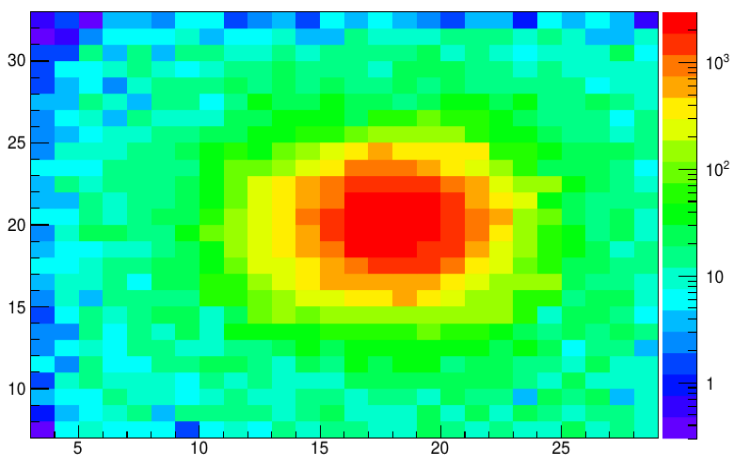
\includegraphics[width=.4\linewidth]{FaisceauSPS1.png}}
					\hfill
					\subfloat{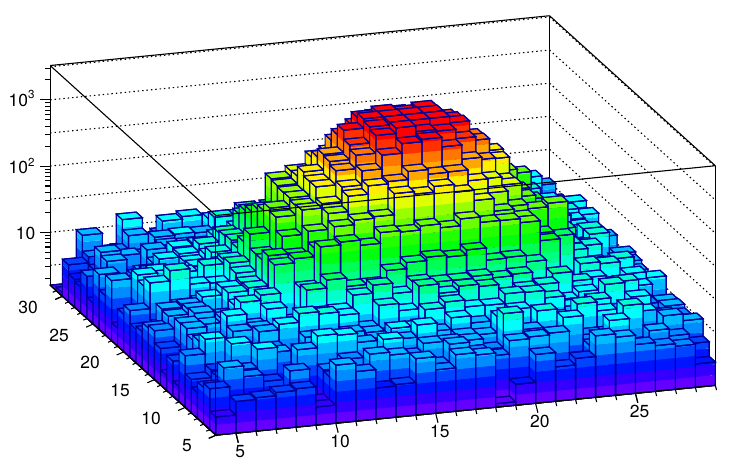
\includegraphics[width=.4\linewidth]{FaisceauSPS2.png}}
				\end{figure}
			\end{columns}
		\end{block}
		\begin{block}{\centering Efficacité et Multiplicité en fonction de la HV}
			\begin{center}
				\scalebox{0.62}{\includetex{HVSPS}}
				
				Le plateau est atteint à $\sim$\SI{6.7}{\kilo\volt} avec une multiplicité de $\sim$\num{2.2}
			\end{center}
		\end{block}
	\end{frame}
	\begin{frame}
	\only<1>{
	\begin{block}{\centering Efficacité en fonction du flux de muons}
		\begin{center}
			\scalebox{1.1}{\includetex{RateSPS}}
		\end{center}
		Les verres de basse résistivité ont une efficacité supérieur à 70\% même à plus de \SI{7}{\kilo\hertz\per\square\centi\meter}.\\
		L'Efficacité du verre "standard" chute brutalement $\sim$40\% à \SI{0.1}{\kilo\hertz\per\square\centi\meter}.
	\end{block}}
	\only<2>{
	\begin{block}{\centering Multiplicité en fonction du flux de muons}
		\begin{center}
		\scalebox{1.1}{\includetex{MultiplicitySPS}}
		\end{center}
	\end{block}}
	\end{frame}
	\subsection{Le GIF++}
	\begin{frame}
		\begin{columns}
			\column{.55\textwidth}
			\begin{block}{\centering Le GIF++}
				\begin{itemize}
					\item Placé sur la ligne H4 du SPS.
					\item Faisceau de muons \SI{150}{\giga\eV}
					\item Source radioactive :  Cs$^{137}$ (\SI{14}{\tera\becquerel}) 
				\end{itemize}
			\end{block}
				\begin{block}{\centering La source radioactive }
					\begin{itemize}
					\item Produit des photons de \SI{661.7}{\kilo\eV}
					\item 2 Atténuateurs indépendants : \\
						3 plans de 3 filtres
						\begin{tabular}{|c|c|c|c|}
						\hline 
						Plan  &A&B&C \\ 
						\hline 
						Position \num{1}&\num{1}&\num{1}&\num{1} \\
						\hline 
						Position \num{2}&\num{10}&\num{1.47}&\num{2.15} \\ 
						\hline 
						Position \num{3}&\num{100}&\num{100}&\num{4.64} \\
						\hline
					\end{tabular} 
				\item Filtre correcteur angulaire : \\
					flux uniforme dans le plan xy
			\end{itemize}
		\end{block}
			\column{.50\textwidth}
			\begin{center}
			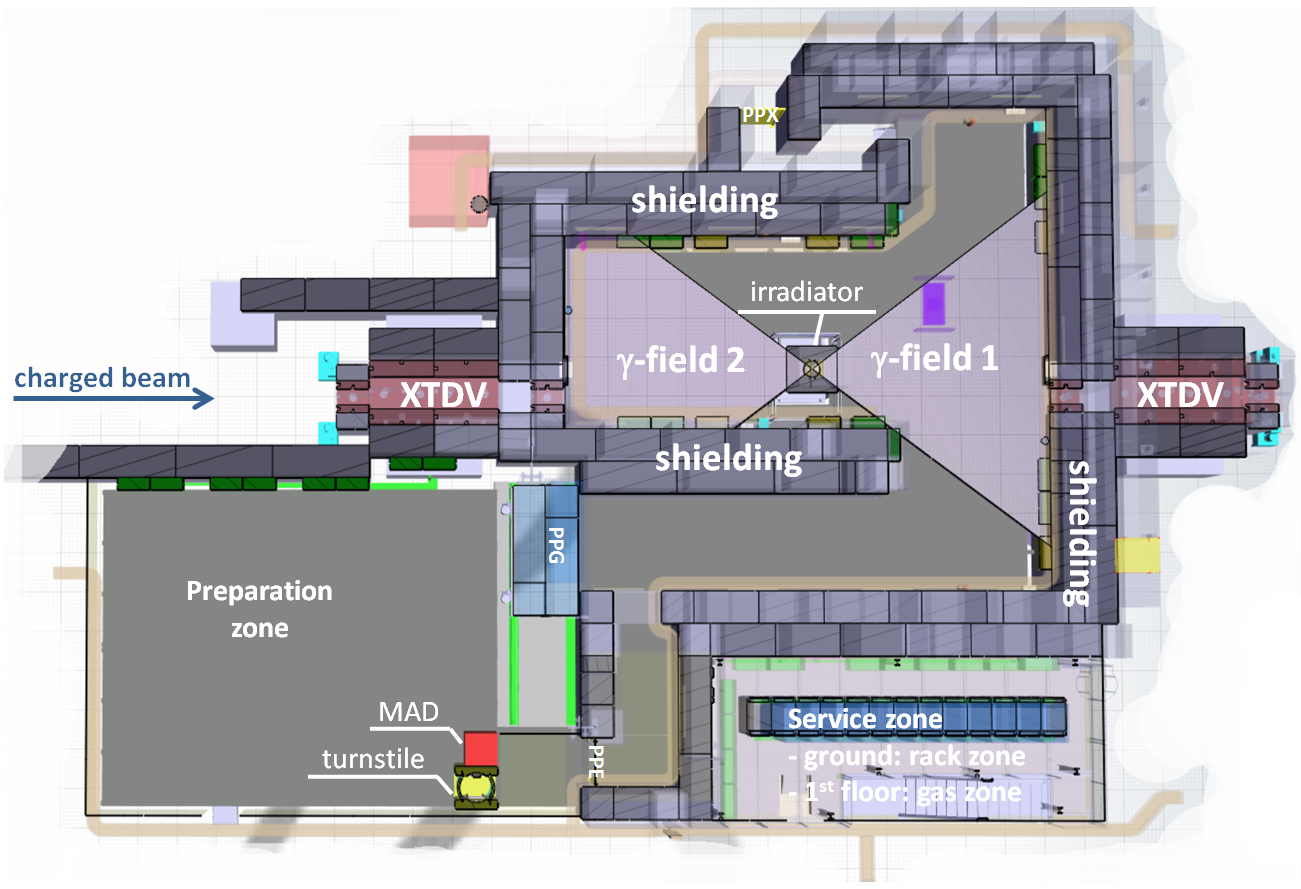
\includegraphics[width=1\linewidth]{GIF1.png}
			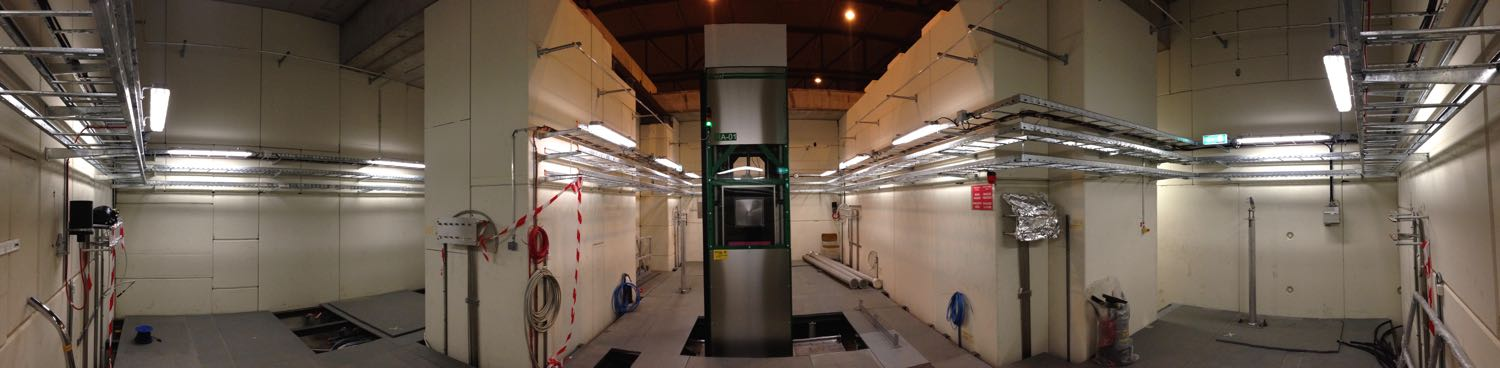
\includegraphics[width=1\linewidth]{GIF3.jpg}
			\end{center}
		\end{columns}
	\end{frame}
	\subsection{Test au GIF++ (Août 2015)}
	\begin{frame}
	\begin{block}{\centering Le télescope}
		\begin{columns}
			\column{.6\textwidth}
			\begin{itemize}
				\item 3 \textit{float glass}/4 Basse résistivité
				\item $\sim$\SI{2}{\meter} de la source
			\end{itemize}
			\column{.40\textwidth}
			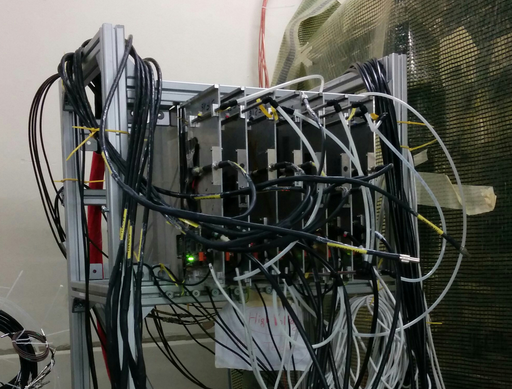
\includegraphics[width=0.5\linewidth]{GIFppChambers.png}\hfill
		\end{columns}
	\end{block}
	\begin{columns}
	\column{.50\textwidth}
	\begin{block}{\centering Flux de gammas au GIF++}
		\begin{center}
		Flux de gamma : $1,5.10^{7}\gamma$\si{\per\square\centi\meter\per\second}
		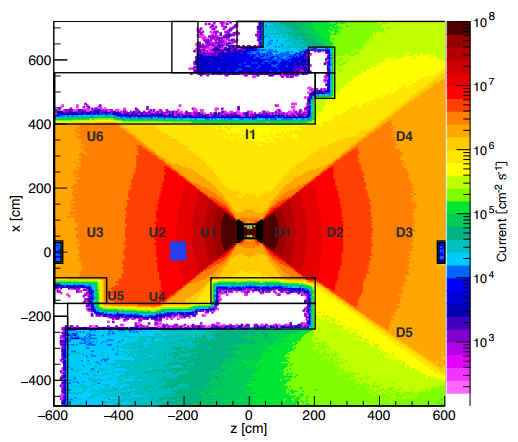
\includegraphics[width=0.8\textwidth]{PositionChamber.png}
		\end{center}
	\end{block}
	\column{.55\textwidth}
	\begin{block}{\centering Taux de conversion $\gamma$/$e^{-}$}
		\begin{center}
		Simulation GEANT4 (verre standard).
		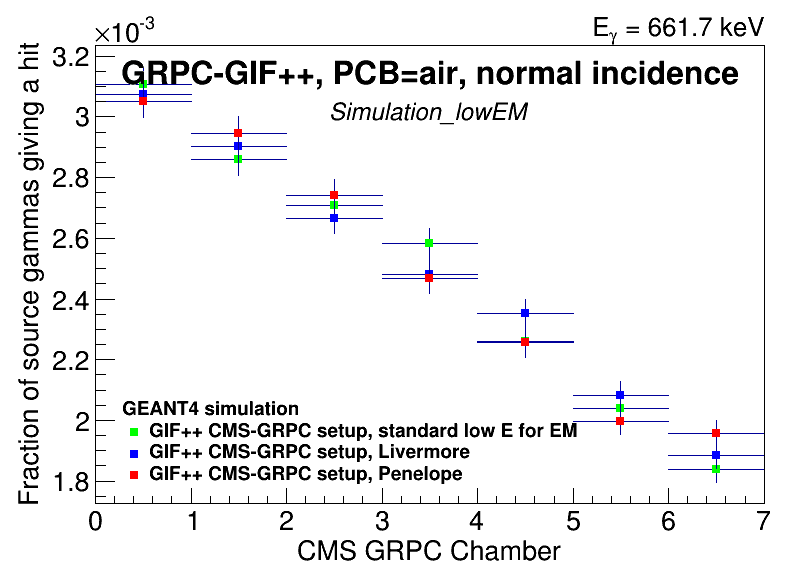
\includegraphics[width=0.8\textwidth]{taux.png}
		\end{center}
	\end{block}
	\end{columns}
	\end{frame}
	\begin{frame}
	\begin{block}{\centering Efficacité en fonction du flux de $\gamma$}
		\begin{center}
		\scalebox{1.1}{\includetex{AttenuateurGIF}}
		L'efficacité des verres de basse résistivité reste supérieur à 70\% pour un flux de $\sim$\SI{2}{\kilo\hertz\per\square\centi\meter}
		\end{center}
	\end{block}
	\end{frame}
	\begin{frame}
	\begin{block}{\centering Courant parcourant les chambres en l'inverse de la valeur d'atténuation}
		\begin{center}
			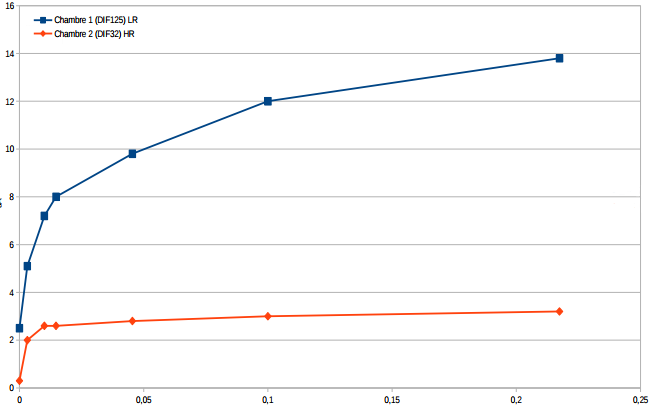
\includegraphics[width=0.8\textwidth]{current_same_HV.png}
		\end{center}
	\end{block}
	\begin{center}
		{\fontsize{9pt}{7.2}\selectfont
	La saturation arrive autour d'un facteur d'atténuation 68.1 pour la float glass.\\
	La chambre en verre de basse résistivité ne semble pas saturer. }
	\end{center}
	\end{frame}
	\subsection{Vieillissement des chambres}
	\begin{frame}
	\begin{center}
	Les chambres doivent supporter une charge intégrée de \SI{1}{\coulomb\per\square\centi\meter}.
	\end{center}
	\begin{block}{\centering Charges intégrées en fonction du nombre de jours effectifs}
			\begin{center}
			Float glass
			\vspace*{-0.6cm}
			\begin{tikzpicture} 
			\node [inner sep=0pt,above right]{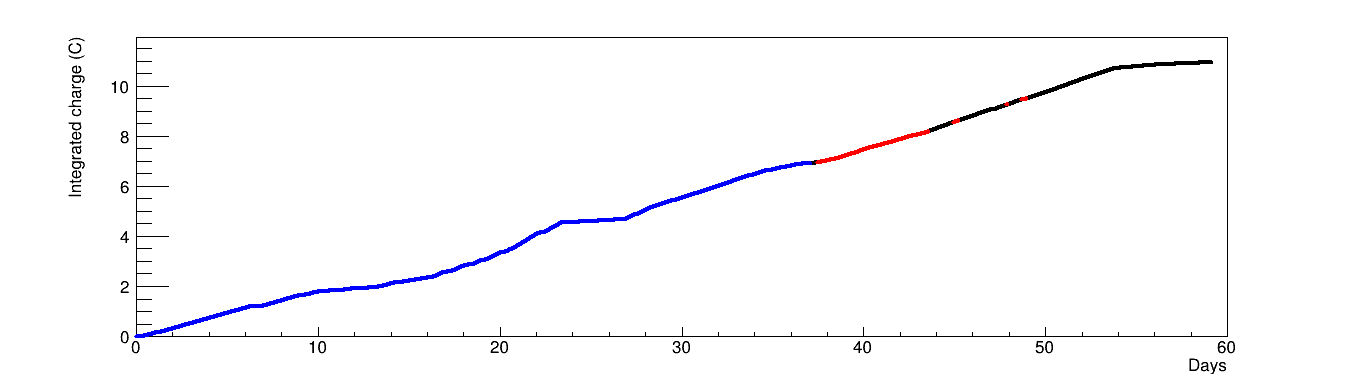
\includegraphics[width=0.98\textwidth]{DIF32_HR_5.png}};
			\path (9.0,2.4) coordinate (vi1);
			\end{tikzpicture} 
		\end{center}
		\begin{center}
			Basse Résistivité
			\vspace*{-0.3cm}
			\begin{tikzpicture} 
			\node [inner sep=0pt,above right]{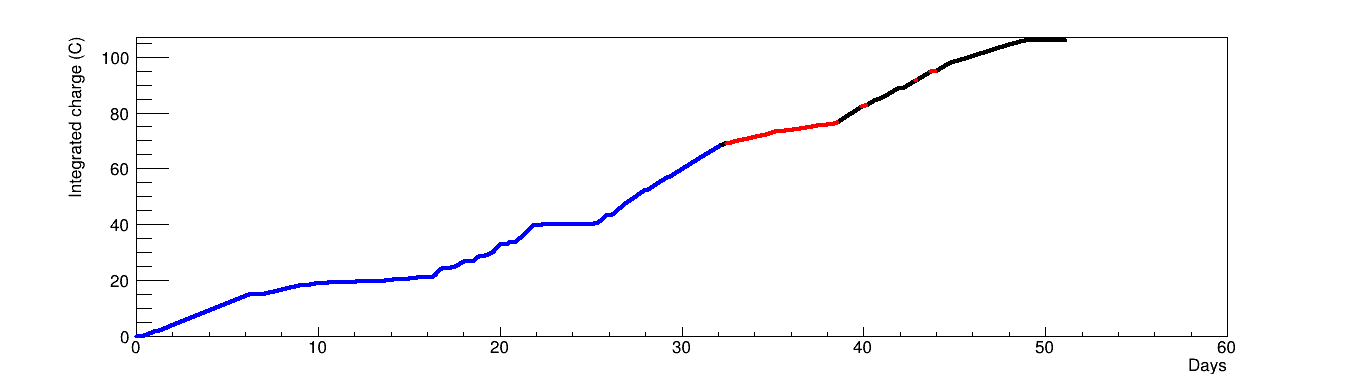
\includegraphics[width=0.98\textwidth]{DIF16_LR_5.png}};
			\path (8.2,2.6) coordinate (vi2);
			\end{tikzpicture} 
			\end{center}
		\visible<2>{\begin{center}
			\vspace*{-0.2cm}
		{\color{red} Vieillissement accéléré !\,\tikz[na] \coordinate (vieil);}
		\end{center}}
	\end{block}
	\begin{tikzpicture}[overlay]
	\draw<2> [thin, red,opacity=.8, fill=red,fill opacity=0.3](vi1) ellipse (15pt and 4pt);
	\path<2>[->,>=latex', red, shorten >=4pt, opacity=.6] (vieil) edge  (vi1);
	\draw<2> [thin, red,opacity=.8, fill=red,fill opacity=0.3](vi2) ellipse (8pt and 4pt);
	\path<2>[->,>=latex', red, shorten >=4pt, opacity=.6] (vieil) edge  (vi2);
	\end{tikzpicture}
	\end{frame}
	\subsection{Test en faisceau au GIF++ (mai-juin 2016)}
	\begin{frame}
	\begin{block}{\centering Mesure à l'argon de la résistivité des électrodes}
			\begin{center}
				\scalebox{0.47}{\includetex{Argon_current}}
			\end{center}	
	\end{block}
		\begin{block}{\centering Estimation de la résistivité}
	\begin{columns}
		\column{.38\textwidth}
		\begin{center}
		$\rho=\frac{RS}{e}$
		\end{center}
		$R$ : résistance de l'électrode \\
		$S$ : Surface des électrodes \\ 
		$e$ : épaisseur des électrodes.
		\column{.55\textwidth}
		\begin{tabular}{|c|c|}
			\hline 
			Chambre 1 (BR)  &\SI{2.4e11}{\ohm.\centi\meter} \\ 
			\hline 
			Chambre 2 (\textit{FG}) & \SI{3.60e12}{\ohm.\centi\meter} \\ 
			\hline 
			Chambre 4 (BR)& \SI{2.49e11}{\ohm.\centi\meter}\\ 
			\hline 
			Chambre 5 (BR) &\SI{3.94e11}{\ohm.\centi\meter} \\
			\hline
		\end{tabular} 
	\end{columns}
	\begin{center}
{\color{red} La résistivité des verres de basses résistivité est beaucoup plus élevé qu'attendue $\sim$\SIrange{1e10}{5e10}{\ohm\centi\meter}}	
	\end{center}
\end{block}	

	\end{frame}
	\subsection{cause du vieillissement prématuré}
	\begin{frame}
	\begin{columns}
	\column{.40\textwidth}
	\begin{block}{\centering Ouverture d'une chambre}
		\begin{center}
	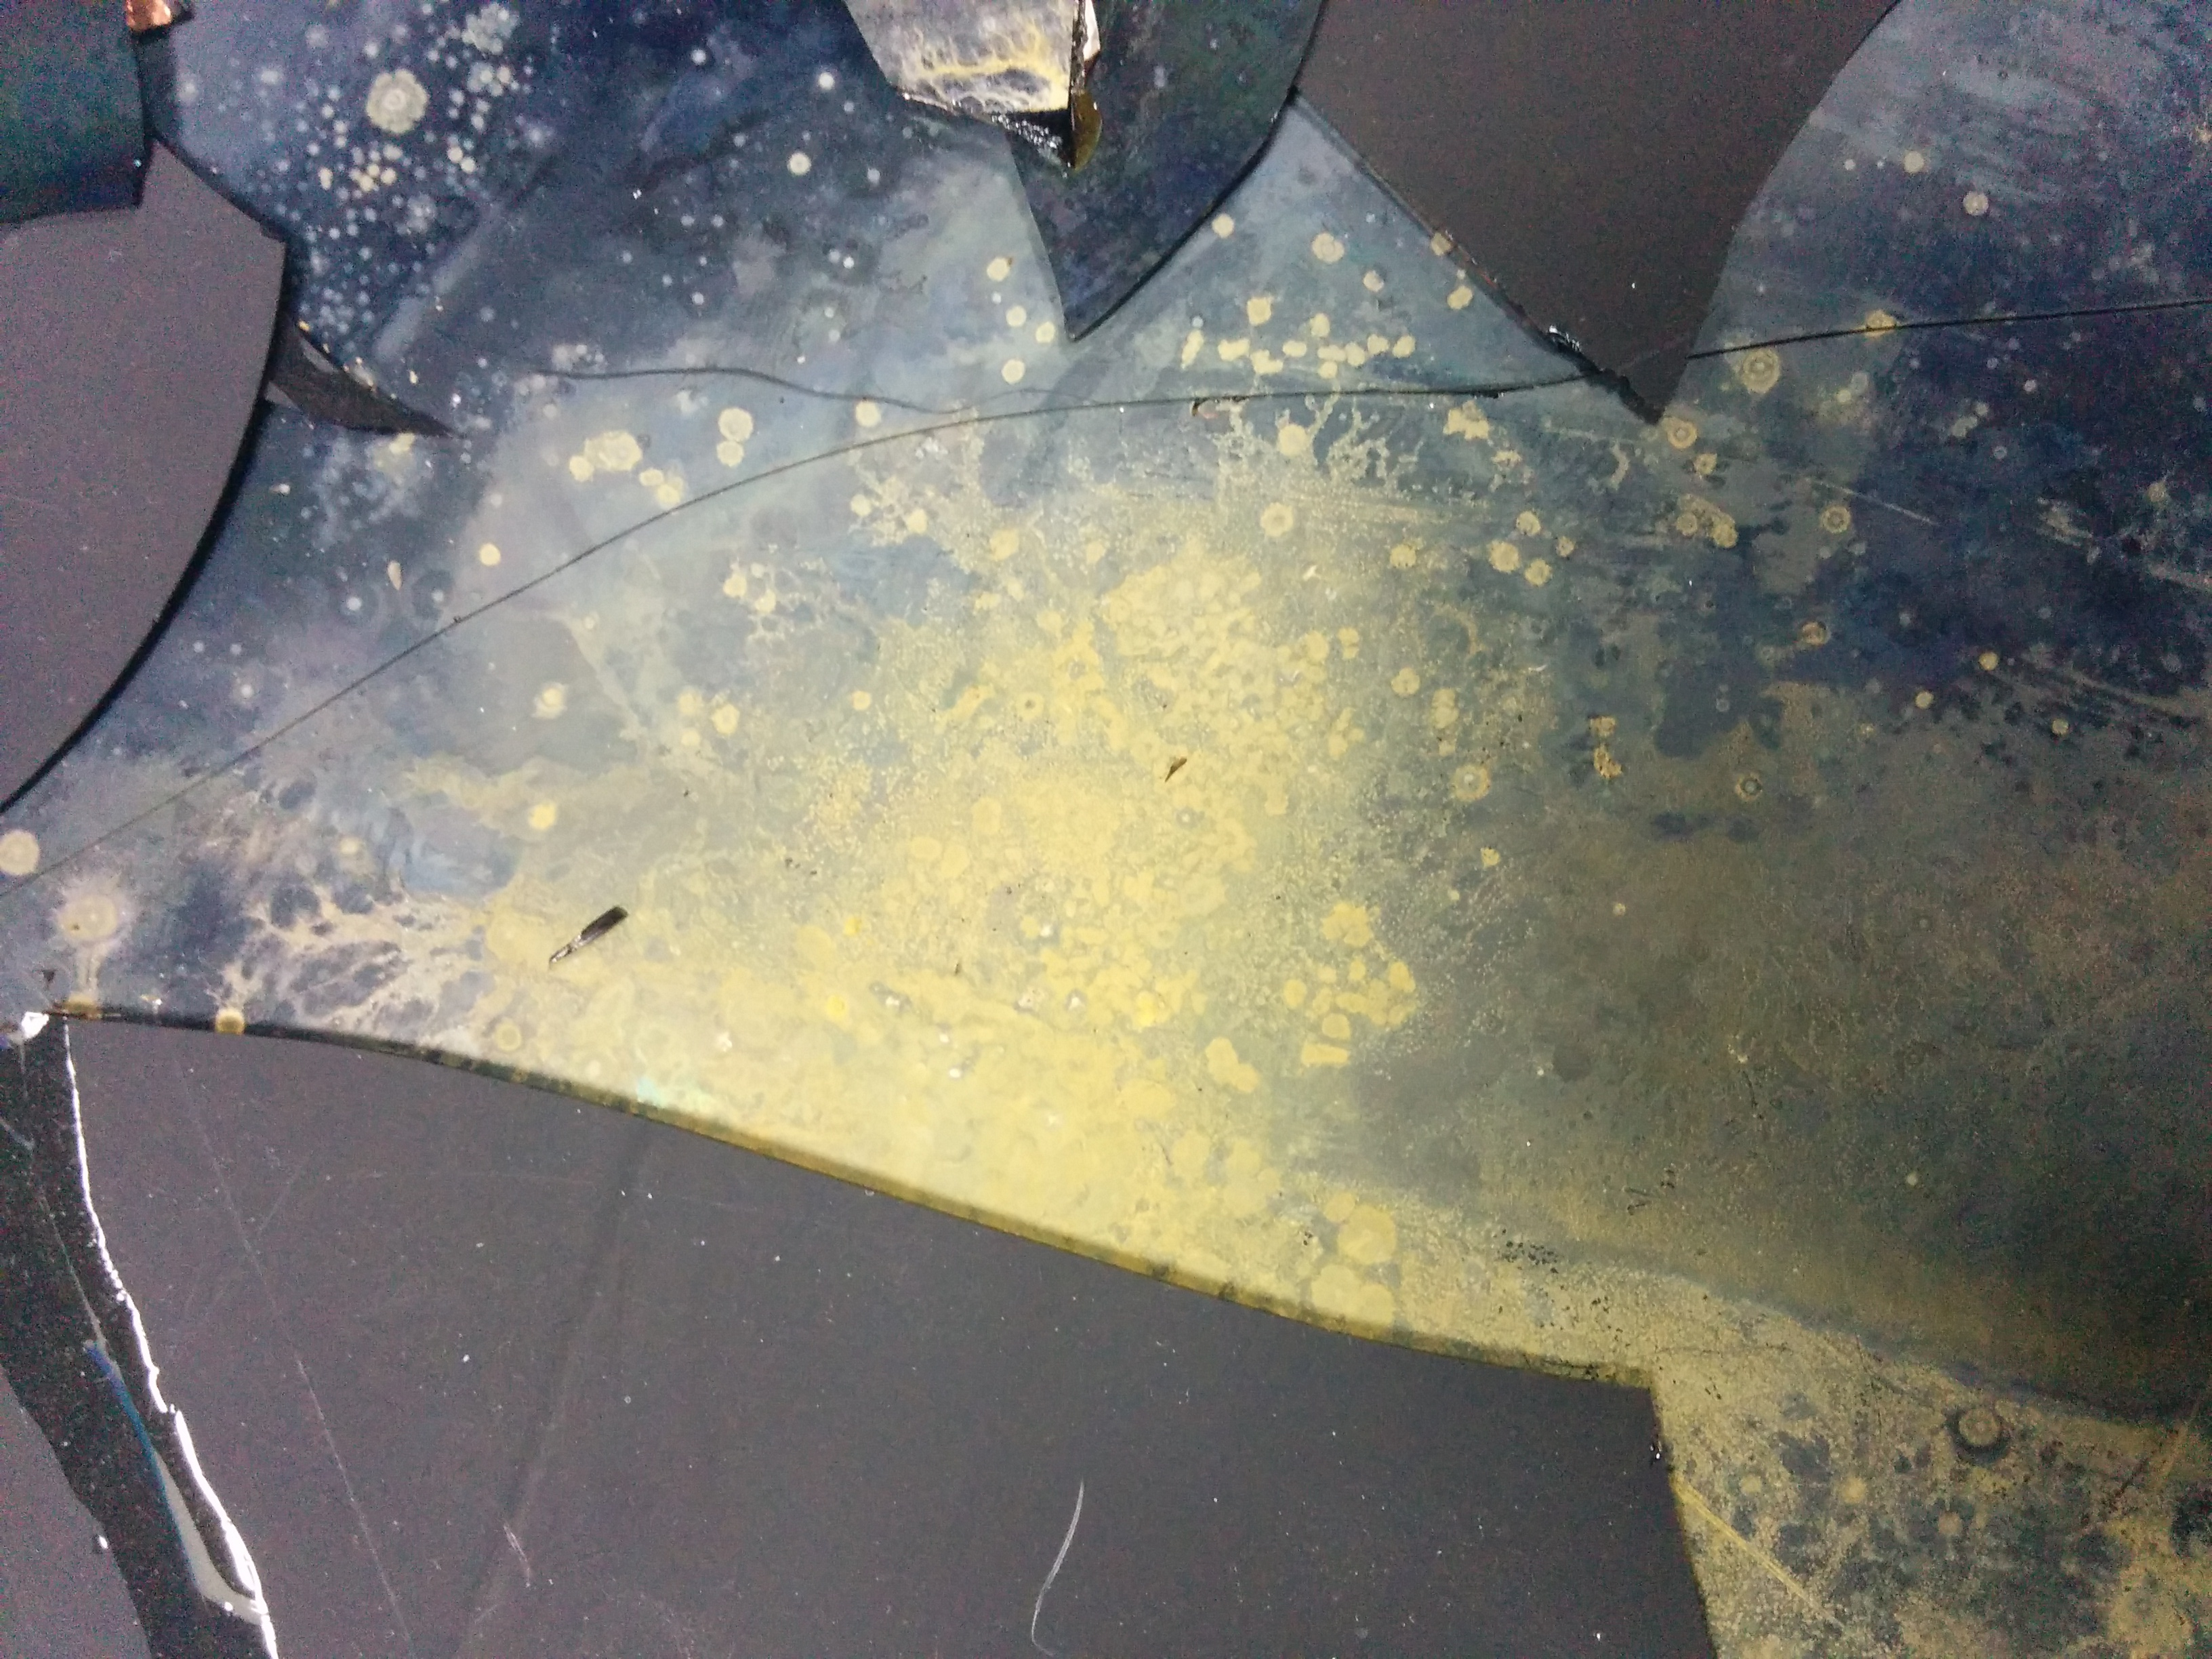
\includegraphics[width=0.5\textwidth]{depot.jpg}
	\end{center}
	\begin{itemize}
		\vspace*{-0.3cm}
	\item Les spacers ont disparus
	\item Formation d'un dépôt
	\end{itemize}
	Explique :
	\begin{itemize}
	\item La résistivité élevée
	\item Les distributions de hits dans l'analyse
	\\
	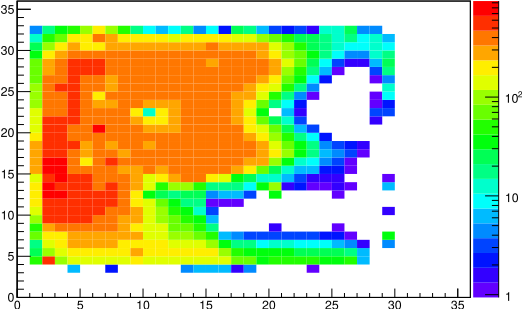
\includegraphics[width=0.25\textwidth]{chamber1.png}
	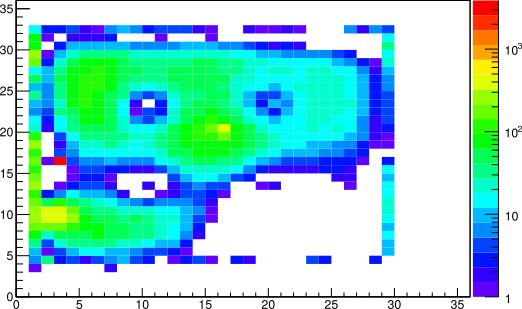
\includegraphics[width=0.25\textwidth]{chamber2.png}
	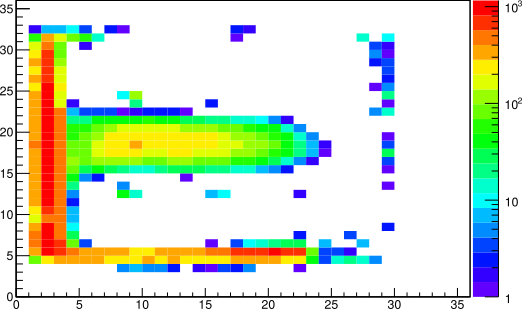
\includegraphics[width=0.25\textwidth]{chamber3.png}
	%\includegraphics[width=0.2\textwidth]{chamber4.png}
	\includegraphics[width=0.25\textwidth]{chamber5.png}
	\end{itemize}
	\end{block}
	\column{.60\textwidth}
	\begin{block}{\centering Causes connues du vieillissement}
		\begin{itemize}
			\item Contamination par l'eau \\
			$\Rightarrow$ Passage de tube en plastique à des tubes en cuivre.
			\item Polymérisation de l'isobutane \\
			$\Rightarrow$ depôt 
			\item Attaque du verre par l'acide fluorhydrique \\
			$\Rightarrow$ dépôt aqueux d'acide fluorosilicique (\chemform{H_2SiF_6}) \\
			%$\Rightarrow$ Diminution de la résistivité et augmentation du taux de bruit.
			\end{itemize}
	\end{block}
	\end{columns}
	\end{frame}
	\section{Chambres de grandes dimensions}
	\subsection{Construction de chambre de grande taille (RE1/1)}
	\begin{frame}
	\begin{center}
	La taille des verre de basse résistivité est limité à \SI{32}{\centi\meter}$\times$\SI{30}{\centi\meter}.
	\end{center}
		\begin{block}{\centering Méthode par collage}
				\begin{columns}
				\column{.45\textwidth}
				\begin{center}
					\includegraphics[width=0.5\textwidth]{Glass-glued.png}
				\end{center}
				\column{.45\textwidth}
				\begin{center}
				\includegraphics[width=0.7\textwidth]{Glass-glued2.png}
				\end{center}
				\end{columns}
				\begin{center}
					Les gaps sont hermétiques.
				\end{center}
				
		\end{block}
		\begin{block}{\centering Méthode par fixation mécanique}
			\begin{columns}
			\column{.45\textwidth}
			\begin{center}
				\includegraphics[width=0.5\textwidth]{meca1.png}
			\end{center}
			\column{.45\textwidth}
			\begin{center}
			\includegraphics[width=0.5\textwidth]{meca2.png}
			\end{center}
		\end{columns}
			\begin{center}
			La cassette est hermétique.
			\end{center}
		\end{block}
	\end{frame}

\subsection{Comparaison des des méthodes d'assemblage}
\begin{frame}
\begin{block}{\centering Comparaison des deux méthodes sur un banc cosmique (verre standard)}
	\begin{center}
	\scalebox{0.9}{\includetex{BigChambersComparaison}}
	
	Les deux méthodes sont comparables.\\
	Le choix s'est porté sur la méthode par fixation mécanique :
	\begin{itemize}
		\item Pas de colle qui pourrait vieillir avec les radiations
		\item Casette hermétique
		\item Pas de gonflements des gaps.
	\end{itemize} 
	\end{center}
\end{block}
\end{frame}

\subsection{Tests en faisceaux au SPS}
\begin{frame}
\begin{columns}
	\column{0.5\textwidth}
	\begin{block}{\centering Setup}
		\begin{itemize}
			\item 2 chambres RE1/1 
			\includegraphics[width=0.60\textwidth]{ChamberFloat.png}
			\item Fixation mécanique
			\item 1 verre standard
			\item 1 verre basse résistivité
			\item gas ILC
			\item Électronique CMS (FEB,DB)
			%\includegraphics[width=0.2\textwidth]{FEBplexis.png}
			\item DAQ utilisé par CMS au GIF++ (TDC)
		\end{itemize}
	\end{block}
	\column{0.5\textwidth}
	\begin{block}{\centering Bruit en fonction de la tension}
		\begin{center}
			\includegraphics[width=0.55\textwidth]{HVNOISEH2.png}
		\end{center}
	\end{block}
	%\begin{block}{\centering Bruit en fonction du seuils}
	%	\begin{center}
	%\includegraphics[width=0.55\textwidth]{THNOISEH2.png}
	%\end{center}
	%\end{block}
\end{columns}
\begin{center}
	Bruit très important $\sim\SI{e5}{\hit\per\strip\per\second}$ pour le verre basse résistivité.
	Réduction d'un facteur $\sim100$ après amélioration du câblage.
\end{center}
\end{frame}
\subsection{Amélioration de la chambre RE1/1}
\begin{frame}
\begin{columns}
	\column{0.5\textwidth}
	\begin{block}{\centering Améliorations}
		\begin{itemize}
			\item FEB approchés du plan de masse
			\item Meilleur masse entre les FEB et le capot
			\item Amélioration du câblage
			\item Remplacement des câbles à l'intérieur de la chambre par des câbles coaxiaux.
		\end{itemize}
	\end{block}
	\column{0.5\textwidth}
	\begin{block}{}
		\includegraphics[width=1\textwidth]{OLDINT.png}
		\includegraphics[width=1\textwidth]{NEWINT.png}
	\end{block}
\end{columns}

\end{frame}
\subsection{Résultats du beam test GIF++ (octobre 2016)}
\begin{frame}
\begin{block}{\centering Efficacité en fonction de la HV}
	\begin{center}
	\scalebox{0.90}{\includetex{SigmoidBC}}
	\end{center}
\end{block}
\end{frame}
\begin{frame}
\begin{block}{\centering Cluster Size en fonction de la tension}
	\begin{center}
	\scalebox{0.90}{\includetex{ClusterSizeBC}}
	\end{center}
\end{block}
\end{frame}
\begin{frame}
\begin{block}{\centering Probabilité de streamer}
	\begin{center}
		Probabilité définit comme la probabilité d'avoir un cluster de taille supérieur à 7.
	\end{center}
\begin{center}
	\scalebox{0.88}{\includetex{ProbaStreamerBC}}
	\end{center}
\end{block}
\end{frame}
\subsection{Étude du bruit en fonction de la proportion de SF6}
\begin{frame}
\begin{columns}
	\column{0.5\textwidth}
	\begin{block}{\centering Taux de bruit dans la chambre RE1/1 vs \% SF6}
		\scalebox{0.4}{\includetex{CurrentRE11}}
	\end{block}
	\column{0.5\textwidth}
	\begin{block}{\centering Taux de bruit dans la double gap 32$\times$30\si{\square\centi\meter} vs \% SF6}
		\scalebox{0.4}{\includetex{EffiNoiseChi}}
		
	\end{block}
\end{columns}
\end{frame}
\subsection{Conclusion}
\begin{frame}
\begin{block}{\centering Conclusion}
\begin{itemize}
	\item Chambres testées sur de nombreuses lignes de faisceaux (DESY,PS,SPS) et au GIF++.
	\item Testées avec différents mélange gazeux (ILC,CMS) et divers proportion de SF6.
	\item Testées avec différentes cellules de lecture (pads,strips) et single, double gaps.
	\item Les verres de basse résistivité sont capable de supporter le flux présent dans les zones RE3/1 et RE4/1.
	\item Il est possible de construire des chambres de grande dimensions avec les verres de basse résistivité de 32$\times$30\si{\square\centi\meter} (2 méthodes)
	\item Le pourcentage de SF6 semble déterminant pour ce type de chambre.
	\item Le vieillissement des chambres n'a pas pu être aboutit.
\end{itemize}
\end{block}
\end{frame}

	\section{L'électronique pour les iRPC}
	\subsection{Principe de la nouvelle Électronique}
	\begin{frame}
	\begin{block}{\centering Principe de la nouvelle Électronique}
		Les strips font toute la longueur de la chambre
	\begin{itemize}
		\item Pas de segmentation en $\eta$ (A,B,C)
		\item Lecture des deux côtés pour le mesurer la position le long du strip 
		\begin{equation}
		Y=\frac{L}{2}-\frac{v(T_2-T_1)}{2}
		\end{equation} 
		$Y$ la position du \textit{hit},$L$ la longueur de la ligne, \\
		$T_1$ et $T_2$ le temps de propagation du signal pour rejoindre l'un et l'autre côté de la ligne, \\
		$T$ le temps d'arrivée du signal sur le \textit{strip} \\ $v$ la vitesse de propagation du signal.
	\end{itemize}
	\begin{center}
	\includegraphics[width=0.50\textwidth]{PCB1.png}
	\end{center}
	\end{block}
	\end{frame}
	\subsection{Le prototype}
	\begin{frame}
	\begin{block}{\centering Le prototype}
		\begin{columns}
		\column{0.50\textwidth}
		\begin{itemize}
			\item \SI{50}{\centi\meter} de long
			\item 32 strips espacés de \SI{4}{\milli\meter}
		\end{itemize}
	\column{0.50\textwidth}
	\begin{center}
		\includegraphics[width=0.45\textwidth]{PCB2.png}
	\end{center}
	\end{columns}
	\end{block}
		\begin{columns}
			\column{0.50\textwidth}
			\begin{block}{\centering Électronique}
				\begin{itemize}
					\item 2 PETIROC (32 vois chacun).
					\begin{center}
					\includegraphics[width=0.35\textwidth]{PETIROC.png}
					\end{center}
					\item 2 TDC (24 voies chacun).
					\begin{center}
					\includegraphics[width=0.35\textwidth]{TDC.png}
					\end{center}
				\end{itemize}
			\end{block}
			\column{0.50\textwidth}
		\begin{block}{\centering Résolution temporelle du PCB}
			\begin{itemize}
				\item Injection d'un signal carré de \SI{10}{\volt} et de durée \SI{10}{\nano\second} à travers un condensateur de \SI{1}{\pico\farad}
				\item $\frac{\sigma_{T_1+T_2}}{\sqrt{2}}=\sigma_{elec}=\num{30.8}\pm\num{0.5}\si{\pico\second}$.
				\begin{center}
					\scalebox{0.40}{\includetex{TDCTimeResolution}}
				\end{center}
			\end{itemize}
		\end{block}
		\end{columns}
	
	\end{frame}
	\subsection{Résolution temporelle de l'électronique}
	%\begin{frame}
%
%\end{frame}
%\subsection{Test en faisceau SPS mai 2017}
\begin{frame}
				\begin{block}{\centering Setup }
						\begin{columns}
						\column{0.50\textwidth}
			\begin{itemize}
				\item Chambre Bakélite gap : \SI{1.4}{\milli\meter} électrodes : \SI{1.4}{\milli\meter}
				%\item Chambre Bakélite gap:\SI{1.6}{\milli\meter} électrode:\SI{1.6}{\milli\meter}
				%\item PCB identique au prototype
				\item Posée sur une table de positionnement.
			
			\end{itemize}
			\column{0.50\textwidth}
		\begin{center}
			\includegraphics[width=0.45\textwidth]{setup2017.jpg}
		\end{center}
	\end{columns}
		\end{block}
	\begin{block}{\centering Résolution temporelle T2-T1}
		\begin{center}
		\includegraphics[width=0.40\textwidth]{25p5cm.png}
		\end{center}
	\end{block}
\end{frame}
\subsection{Résolution Spatiale}
\begin{frame}
\begin{block}{\centering Résolution Spatiale}
	\begin{center}
	\includegraphics[width=0.76\textwidth]{MeanT_Pos.png}
	\end{center}
	\begin{center}
	$<\Delta T>=<T_2-T_1>$ en fonction de la position $Y$ du détecteur.
	\end{center}
	\begin{center}
	$v=2\frac{\diff Y}{\diff <\Delta T>}=2*\frac{1}{0.11}=\SI{18.18}{\centi\meter\per\nano\second}$
	\end{center}
	$=> \sigma_{Y}=\sigma_{T_2-T_1}\frac{v}{2}\approx\SI{1.8}{\centi\meter}$
\end{block}
\end{frame}
	\section{Conclusion et perspectives}
	\begin{frame}
	\begin{block}{\centering Conclusion et perspectives}
		Blabla
	\end{block}
	\end{frame}








































\appendix
\section{Backup}
\subsection{Le Modèle Standard}
\begin{frame}
\begin{block}{\centering Le modèle standard}
	\begin{itemize}
		\item Théorie non-abélienne
		\item Théorie perturbative
		\item Théorie quantique des champs (relativiste et quantique)
		\item l'ensemble des informations de la théorie est contenue dans un Lagrangien $\mathcal{L_{MS}}$
	\end{itemize}
\end{block}
\begin{block}{\centering Lagrangien du Modèle Standard}
	\begin{equation}
	\mathcal{L_{MS}}=\mathcal{L}_{\mathrm{Yang-Mills}}+\mathcal{L}_{\mathrm{Dirac}}+\mathcal{L}_{\mathrm{Higgs}}+\mathcal{L}_{\mathrm{Yukawa}}
	\end{equation}
	\begin{itemize}
		\item $\mathcal{L}_{\mathrm{Yang-Mills}}$ Partie cinétique des champs de jauges.
		
		\item $\mathcal{L}_{\mathrm{Dirac}}$ Interactions entre fermions et bosons de jauges.
		
		\item $\mathcal{L}_{\mathrm{Higgs}}$ Donne la masse aux bosons $Z^{0}$,$W^{\pm}$.
		
		\item $\mathcal{L}_{\mathrm{Yukawa}}$ Interactions entre le boson de Higgs et les fermions.
	\end{itemize}
\end{block}
\end{frame}
\subsection{Succès et lacunes du Modèle Standard}
\begin{frame}
\begin{columns}
\column{.5\textwidth}
\begin{vert}{\centering Ses succès}
	\begin{itemize}
		\item Prédiction du courant neutre
		\item Théorie renormalisable
		\item Excellents accords avec les mesures expérimentales 
	\end{itemize}
	\vspace*{-0.5cm}
	\begin{figure}[ht!]
		\centering
		\includegraphics[width=0.55\textwidth]{mesure.png}
		%\caption{Comparaison des résultats d'ajustement avec les mesures directes de certains paramètres du Modèle Standard.}
	\end{figure}
\end{vert}
\column{.5\textwidth}
\begin{rouge}{\centering Ses lacunes}
	\begin{itemize}
		\item Le nombre de familles
		\item Asymétrie baryon-antibaryons
		\item Gravitation non incluse
		\item Matière Noire et Énergie Noire 
		\begin{center}
			\includegraphics[width=0.50\textwidth]{darkmatter.png}
		\end{center}
		\item Le nombre important de paramètres libres
		\item Neutrinos massifs
		\item non unification des couplages
		\item Naturalité
	\end{itemize}
\end{rouge}
\end{columns}
\end{frame}
\subsection{Au-delà du Modèle Standard}
\begin{frame}
\begin{block}{\centering Modèles au-delà du Modèle standard}
Extension du Modèle Standard :
\begin{itemize}
\item \textit{Grand Unified Theories} : unifier les interactions sous une même symétrie.
Basé sur un groupe $G\supset SU(3)\times SU(2) \times U(1)$
\item Supersymétrie (SuSy) : supprimer le problème de la naturalité en associant à chaque fermions un  boson superpartenaire et réciproquement. 
\begin{figure}
	\centering
	\includegraphics[width=0.60\textwidth]{SuSy.png}
\end{figure}
\item Modèle avec dimensions supplémentaires enroulées.
\end{itemize}
\end{block}
\end{frame}


\subsection{Le complexe d'accélération du CERN}	
\begin{frame}
\begin{columns}
	\column{.5\textwidth}
	\begin{center}
		\includegraphics[width=1.1\textwidth]{complexe.png}
	\end{center}
	\column{.5\textwidth}
	\begin{block}{\centering Pour les collisions proton-proton}
		\begin{itemize}
			\item LINAC 2 ($\SI{50}{\mega\eV}$)
			\item BOOSTER ($\SI{1.4}{\giga\eV}$)
			\item {\only<1>{\color{red}}Synchrotron à protons (PS) ($\SI{25}{\giga\eV}$)}
			\item {\only<2>{\color{red}}SuperSynchrotron à protons (SPS) ($\SI{450}{\giga\eV}$)}
			\item Large Hadron Collider (LHC) ($\SI{7}{\tera\eV}$)
		\end{itemize}
	\end{block}
\end{columns}
\only<1>{\begin{block}{\centering Ligne de faisceaux (East Area)}
		\begin{itemize}
			\item Particules : électrons, hadrons, muons...
			\item quantité de mouvement : \SIrange{1}{15}{\giga\eV}
			\item Intensité du faisceau : $\sim1-2\times 10^{6}$part/Spill
			\item Structure du Spill : 
			\begin{itemize}
				\item \SI{400}{\milli\second} 
				\item 1 Spill toutes les \SI{33}{\second} (ou plus)
			\end{itemize}
		\end{itemize}
\end{block}}
\only<2>{\begin{block}{\centering Ligne de faisceaux (North Area)}
		\begin{itemize}
			\item Particules : électrons, hadrons, muons...
			\item quantité de mouvement : \SIrange{10}{400}{\giga\eV}
			\item Intensité du faisceau : $\sim1-2\times 10^{8}$part/Spill
			\item Structure du Spill : 
			\begin{itemize}
				\item \SIrange{4.8}{9.6}{\second} 
				\item 1 Spill toutes les \SIrange{14}{48}{\second}
			\end{itemize}
		\end{itemize}
\end{block}}
\end{frame}
\begin{frame}
\begin{block}{\centering Électronique}
	\begin{itemize}
		\item Partition en $\eta$ (A,B,C) de 32 strips chacunes. 
		\item 3 Front-End Boards (mise en forme du signal).
		\begin{center}
			\includegraphics[width=0.35\linewidth]{Feb.png}
		\end{center}
		\item Distribution Board (paramètrage des FEBs).
		\begin{center}
			\includegraphics[width=0.30\linewidth]{DB.png}
		\end{center}
	\end{itemize}
\end{block}
\end{frame}
\subsection{Mise à niveau des RPC}
\begin{frame}
\begin{block}{\centering Instrumentation des zone RE3/1 et RE4/1 (1.8<$\eta$<2.4)}
\begin{itemize}
	\item Améliorer la résolution temporelle des traces muons
	\begin{center}
		\includegraphics[width=0.45\linewidth]{intrasec.png}
	\end{center}
	\item recouvrer les zones moins efficaces des CSC
	\begin{center}
		\includegraphics[width=0.32\linewidth]{effstation4.png}
	\end{center}
	\item Augmenter la redondance dans cette zone \\
	En cas de CSC défaillants.
\end{itemize}
\end{block}
\end{frame}
\subsection{Premiers résultats à DESY (janvier 2012)}
\begin{frame}
\begin{columns}
	\column{.6\textwidth}
	\begin{block}{\centering Chambres}
		\begin{itemize}
			\item 5 chambres \\
			\item 1 "float glass", 4 "Basse Résistivité"
			\item Électronique HARDROC 
			\item Pads
		\end{itemize}
	\end{block}
	\begin{block}{\centering Faisceau}
		\begin{itemize}
			\item Électrons (Jusqu'à \SI{6}{\giga\eV})
			\item  Surface de quelques \si{\square\centi\meter}
		\end{itemize}
	\end{block}
	\begin{block}{\centering Mélange gazeux (ILC)}
		\begin{itemize}
			\item 93\% de Tétrafluoroéthane \chemform{C_2H_2F_4}.
			\item \num{5}\% \chemform{CO_2}, absorbeur de photons UV. 
			\item \num{2}\% d'hexafluorure de soufre \chemform{SF_6}, capture l'excès d'électrons.
		\end{itemize}
	\end{block}
	\column{.5\textwidth}
	\begin{center}
		\includegraphics[width=1\textwidth]{effiDesy.png}
	\end{center}
\end{columns}
\end{frame}

\subsection{Programme d'analyse pour les chambres à électronique CMS}
{\fontsize{8pt}{7.2}\selectfont
	\begin{frame}
	\vspace*{-0.3cm}
	\begin{overlayarea}{0.99\textwidth}{8cm}
		\begin{block}{\centering Méthode de suppression du bruit}
			\begin{center}
				Sélection de la zone temporelle du signal:
			\end{center}
			\begin{itemize}
				\item Réalignement des timestamps des hits avec le timestamp moyen de la chambre.
				\item Ajustement de la distribution des hits en fonction du timestamp par une Gaussienne+constante
				%\only<2-3>{\begin{center}\scalebox{0.22}{\includetex{fitting_aligned}}\end{center}}
				\item Sélection de la fenêtre [$\mu$-3$\sigma$,$\mu$-3$\sigma$]
			\end{itemize}
		\begin{center}
					Estimation de l'efficacité réelle:
			\end{center}
			\begin{itemize}
				\item Calcule de l'efficacité dans la zone du signal $\epsilon^{signal}$
				\item Découpe de la partie temporelle avant le signal en intervalles $I_{n}=\left[t_{n}-t_{win},t_{n}+t_{win}\right]$
				\item Calcul de l'efficacité $\epsilon^{bruit}$ et du taux moyens de bruit $\overline{N^{hits}_n}$ dans ces intervalles.
				\item Sélection de $I_{n}$ pour lequel $\overline{N^{hits}_n}$ est maximale.
				\item Calcul de l'estimateur de l'efficacité :$\epsilon=\frac{\epsilon^{signal}-k\epsilon^{bruit}}{1-k\epsilon^{bruit}}$\\
					\begin{equation}
					k=\frac{1-\mbox{Poisson}\left(k=0,\lambda=\frac{\overline{N^{hits}_{max}}T^{signal}}{T^{bruit}}\right)}{1-\mbox{Poisson}\left(k=0,\lambda=\frac{\overline{N^{hits}_{max}}}{T^{bruit}}\right)}
					\end{equation}	
			\end{itemize}
		\end{block}
	\end{overlayarea}
\end{frame}}
\subsection{Test de la méthode de suppression du bruit}
\begin{frame}
\begin{overlayarea}{0.99\textwidth}{8cm}
\only<1>{
	\begin{block}{\centering Biais de l'estimateur $\epsilon$}
		Monte Carlo : 50 000 triggers pour chaque paire $\left(\epsilon^{signal},\epsilon^{bruit}\right)$  ($T_{signal}=3\times T_{bruit}$).
		\begin{center}
		\scalebox{0.4}{\includetex{biais2}}\end{center}
\end{block}}
\only<2>{\begin{block}{\centering Écart-type de l'estimateur $\epsilon$}
		Monte Carlo : 2 500 000 expériences réparties dans 50$\times$50 bins.
		
		\begin{center}\scalebox{0.5}{\includetex{std}}\end{center}
\end{block}}
\end{overlayarea}
\end{frame}

\subsection{Le SDHCAL}
\begin{frame}
\begin{columns}
	\column{0.7\textwidth}
	\begin{block}{\centering Prototype SDHCAL}
		\begin{columns}
			\column{0.45\textwidth}
		Calorimètre hadronique Semi-digital pour ILD.
				\begin{itemize}
			\item \SI{1}{\cubic\meter}
			\item 48 GRPC "verre standard"
		\end{itemize}
		\column{0.45\textwidth}
		\begin{center}
		\includegraphics[width=1\textwidth]{SDHCAL.jpg}
		\end{center}
	\end{columns}
	\end{block}
	\column{0.3\textwidth}
	\begin{block}{\centering International Large Detector}
		\begin{center}
		\includegraphics[width=0.80\textwidth]{ILD.png}
		\end{center}
	\end{block}
\end{columns}
\begin{block}{\centering International Linear Collider}
	\begin{center}
	\includegraphics[width=0.6\textwidth]{ILC.png}
	\end{center}
\end{block}
\end{frame}
\end{document}
